\documentclass[11pt]{article}

\usepackage{sectsty}
% \usepackage{graphicx}
\usepackage{multirow}
\usepackage{abstract}
\usepackage[final]{graphicx}
\usepackage{subcaption}
% \usepackage{subfig}
\usepackage{float}


\renewcommand{\contentsname}{\centering Contents}   
\renewcommand{\abstractnamefont}{\normalfont\normalsize\bfseries\Large}
\renewcommand{\abstracttextfont}{\large}

% Margins
\topmargin=-0.45in
\evensidemargin=0in
\oddsidemargin=0in
\textwidth=6.5in
\textheight=9.0in
\headsep=0.25in

% \title{Monte Carlo Tree Search driven Falsification}
\title{Temporal Logic Falsification via Monte Carlo Tree Search}
\author{Lugi Berducci \and Alessandro Steri}
\date{\today}

\begin{document}
\maketitle	


%--Paper--
\begin{abstract}
Simulation-based verification is often the only chance to verify complex hybrid systems and it requires a large amount of time and resources.
In particular, the process to find anomalies and faults is called \textit{falsification} because it consists of finding a scenario (a trace of disturbances) that leads the system to violate the requirements, described as formal specifications.

Many research groups are focusing their effort on techniques for reduction of verification time and recent works adopted search algorithms driven by a heuristic called \textit{robustness}.

In this project, we focused on falsification of Temporal Logic Specification using one of the most promising search algorithm: the Monte Carlo Tree Search, famous for being adopted in AlphaGo. Specifically, we tested this approach on the well-known Automatic Transmission model and analysed the obtained result, describing strenghts and difficulties of MCTS algorithm.

\end{abstract}

% Optional TOC
\tableofcontents

\pagebreak

\section{Two-Layered Falsification}
\subsection{Introduction}
The process of falsification aims to find a counter example to a given specification, such examples typically are \textit{hard to find} errors. In general, the search space is too wide and the process of verification through simulation is expensive, thus a clever strategy to drive the search and properly invest the simulation time is crucial.

Following the work done in \cite{zhang2018two} we decided to use a two layer strategy. In the top layer, Monte Carlo Tree Search act as a zoomed out view of the search: at each control point, the system quantizes the input space in regions and tries to iteratively explore new regions and give to those region a score mesuring how promising they are (see Section~\ref{sec:MCTS}). 
In the bottom layer, a search algorithm (see Section~\ref{sec:srcalg}) starts a fine grain exploration in the promising regions coming from the top layer and updates score.

Whilst the MCTS allows to tune the tradeoff between exploration and exploitation at a macroscopic level, the second layer algorithm works only on a few selected regions according to the time advance.

Given the success of MCTS in automated game play, this approach seems to be promising in verification because of its adversarial characterization. In fact, we could interpret the verification problem as if the error is cleverly placed by an adversary and the strategy needs to be clever enough to find it. 

\subsection{Upper-layer: MCTS}~\label{sec:MCTS}
The MCTS is based on the iterative building of a tree $T=(V,E)$ where nodes $v \in V$ are labelled with a score $v.s$ and a counter $v.n$, and edges in $E$ are labelled with the corresponding actions. At the begin, the tree is initialized as a root node with $root.s=Inf$ and $root.n=0$.
The execution evolves in different phases described below and represented by the Figure~\ref{fig:mcts}.

\begin{figure}[H]
  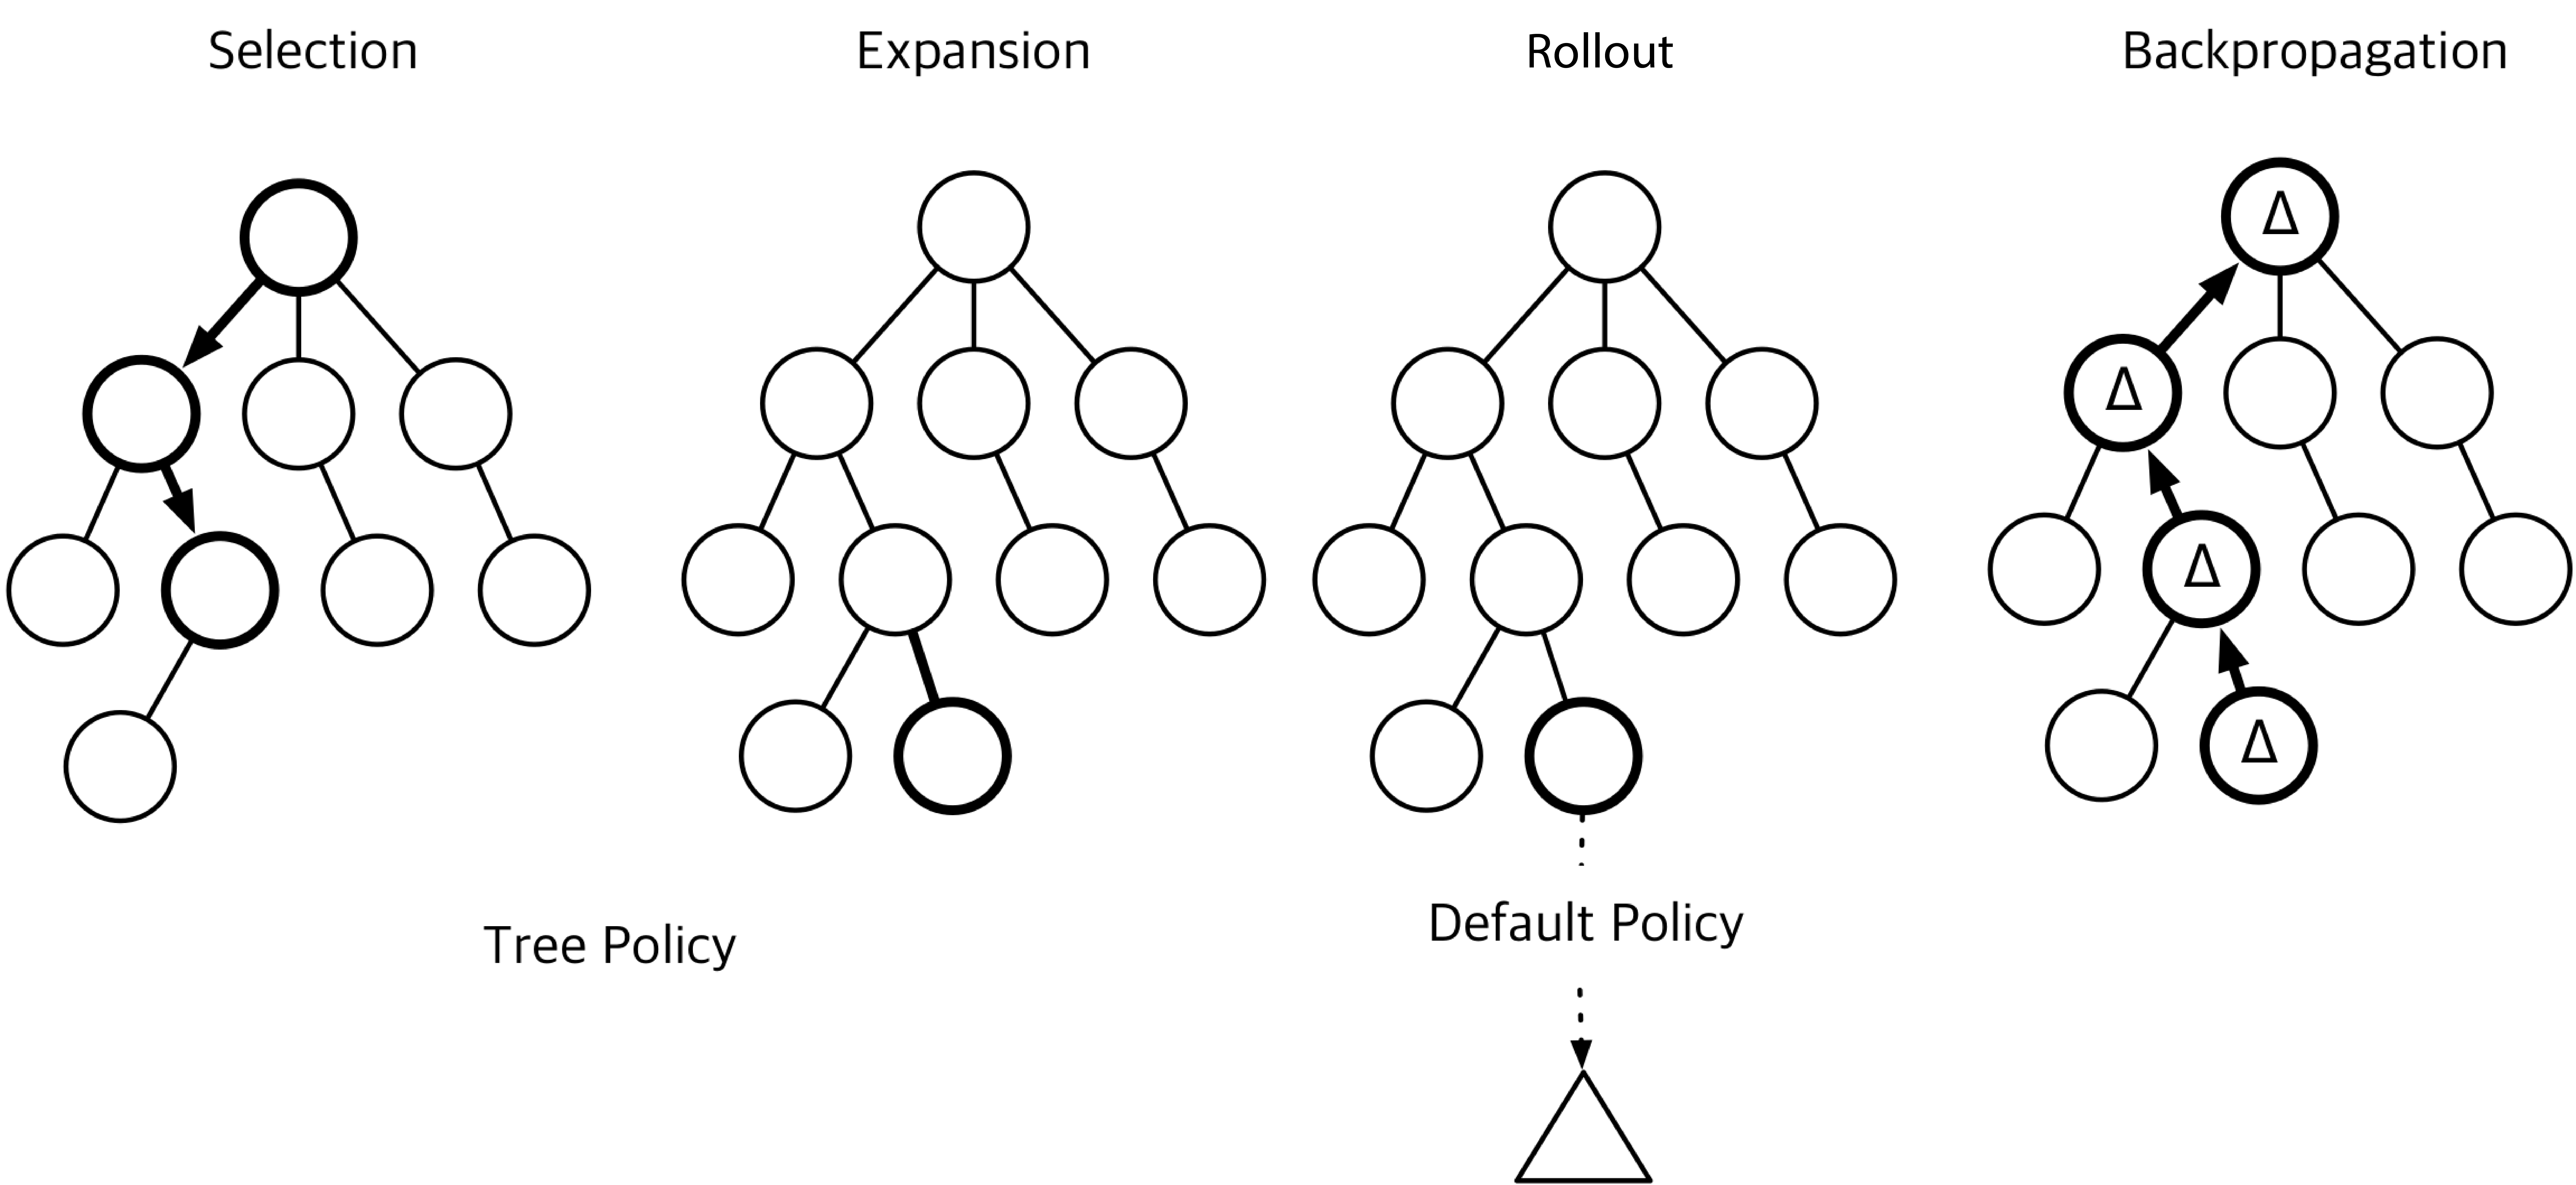
\includegraphics[width=\linewidth]{img/mcts2.png}
  \caption{Graphical overview of MCTS phases and theirs behaviors.}
  \label{fig:mcts}
\end{figure}

\paragraph{Selection:} Visit the tree starting from the root, moving to the node $v$ which maximize the UCB($v$) function explained in the following paragraph.
Once a leaf $l$ is reached, if the tree hasn't yet reached its maximum expansion (i.e. the height of the tree corresponds to the control points in the simulation) then go to Expansion($l$), otherwise it directly run Rollout($l$).

\paragraph{Expansion:} For each action $a$ available from $l$ we expand the tree $T$ with a new node $v$ having $v.s=Inf$, $v.n=0$ and connected to the node $l$ through an edge labeled $a$. Finally, we pick a random child $c$ of $l$, and run Rollout($c$).

\paragraph{Rollout(l)} For each ancestor node of $l$ starting from the root till $l$ itself, the lower layer (see Section~\ref{sec:srcalg}) searches in the region of the selected node (tree policy). Then starting from the leaf $l$, the remaining simulation is driven by the search (default policy) up till the horizon. At the end, the trace will have a robustness value of $s$ which will be used as an estimate for $l$ and its ancestors by means of Backpropagation($l,s$).

\paragraph{Backpropagation(l,s):} From $l$ till the root, going trough $l$'s ancestors say $l=a_1, a_2, \dots, a_n=root$, update each $a_i$ as follow:
\begin{itemize}
    \item $a_i.n=a_i.n + 1$
    \item $a_i.s=min\{a_i.s, s\}$
\end{itemize}

\paragraph{UCB(v):} In the most general MCTS implementation, the UCB value of the node $v$ is computed as:

\begin{equation}
    UCB = v.s + C \cdot \sqrt{\frac{\ln N}{v.n}}
\end{equation}
where $N = root.n$ hence the total number of visited nodes. The idea behind the parameter $C$ (see Figure~\ref{fig:C}) is to fine-tune exploration (see \ref{fig:c1}) vs exploitation (see \ref{fig:c0}). 

When considering the falsification problem thus using robustness as heuristic we face two problem:
\begin{itemize}
    \item Robustness can have positive yet negative values while classical UCB is designed to work with only positive value. 
    \item Generally, given a specification it is not possible to give an upper bound to the robustness domain. 
\end{itemize}
To overcome both the problems, along the line of \cite{zhang2018two}, we used UCT defined as:

\begin{equation}
    UCT = 1 - \frac{v.s}{max_v v.s} + C \cdot \sqrt{\frac{\ln N}{v.n}}
\end{equation}
% \pagebreak


% \begin{figure}[H]
% \begin{subfigure}{\textwidth}
%   \centering
%   % 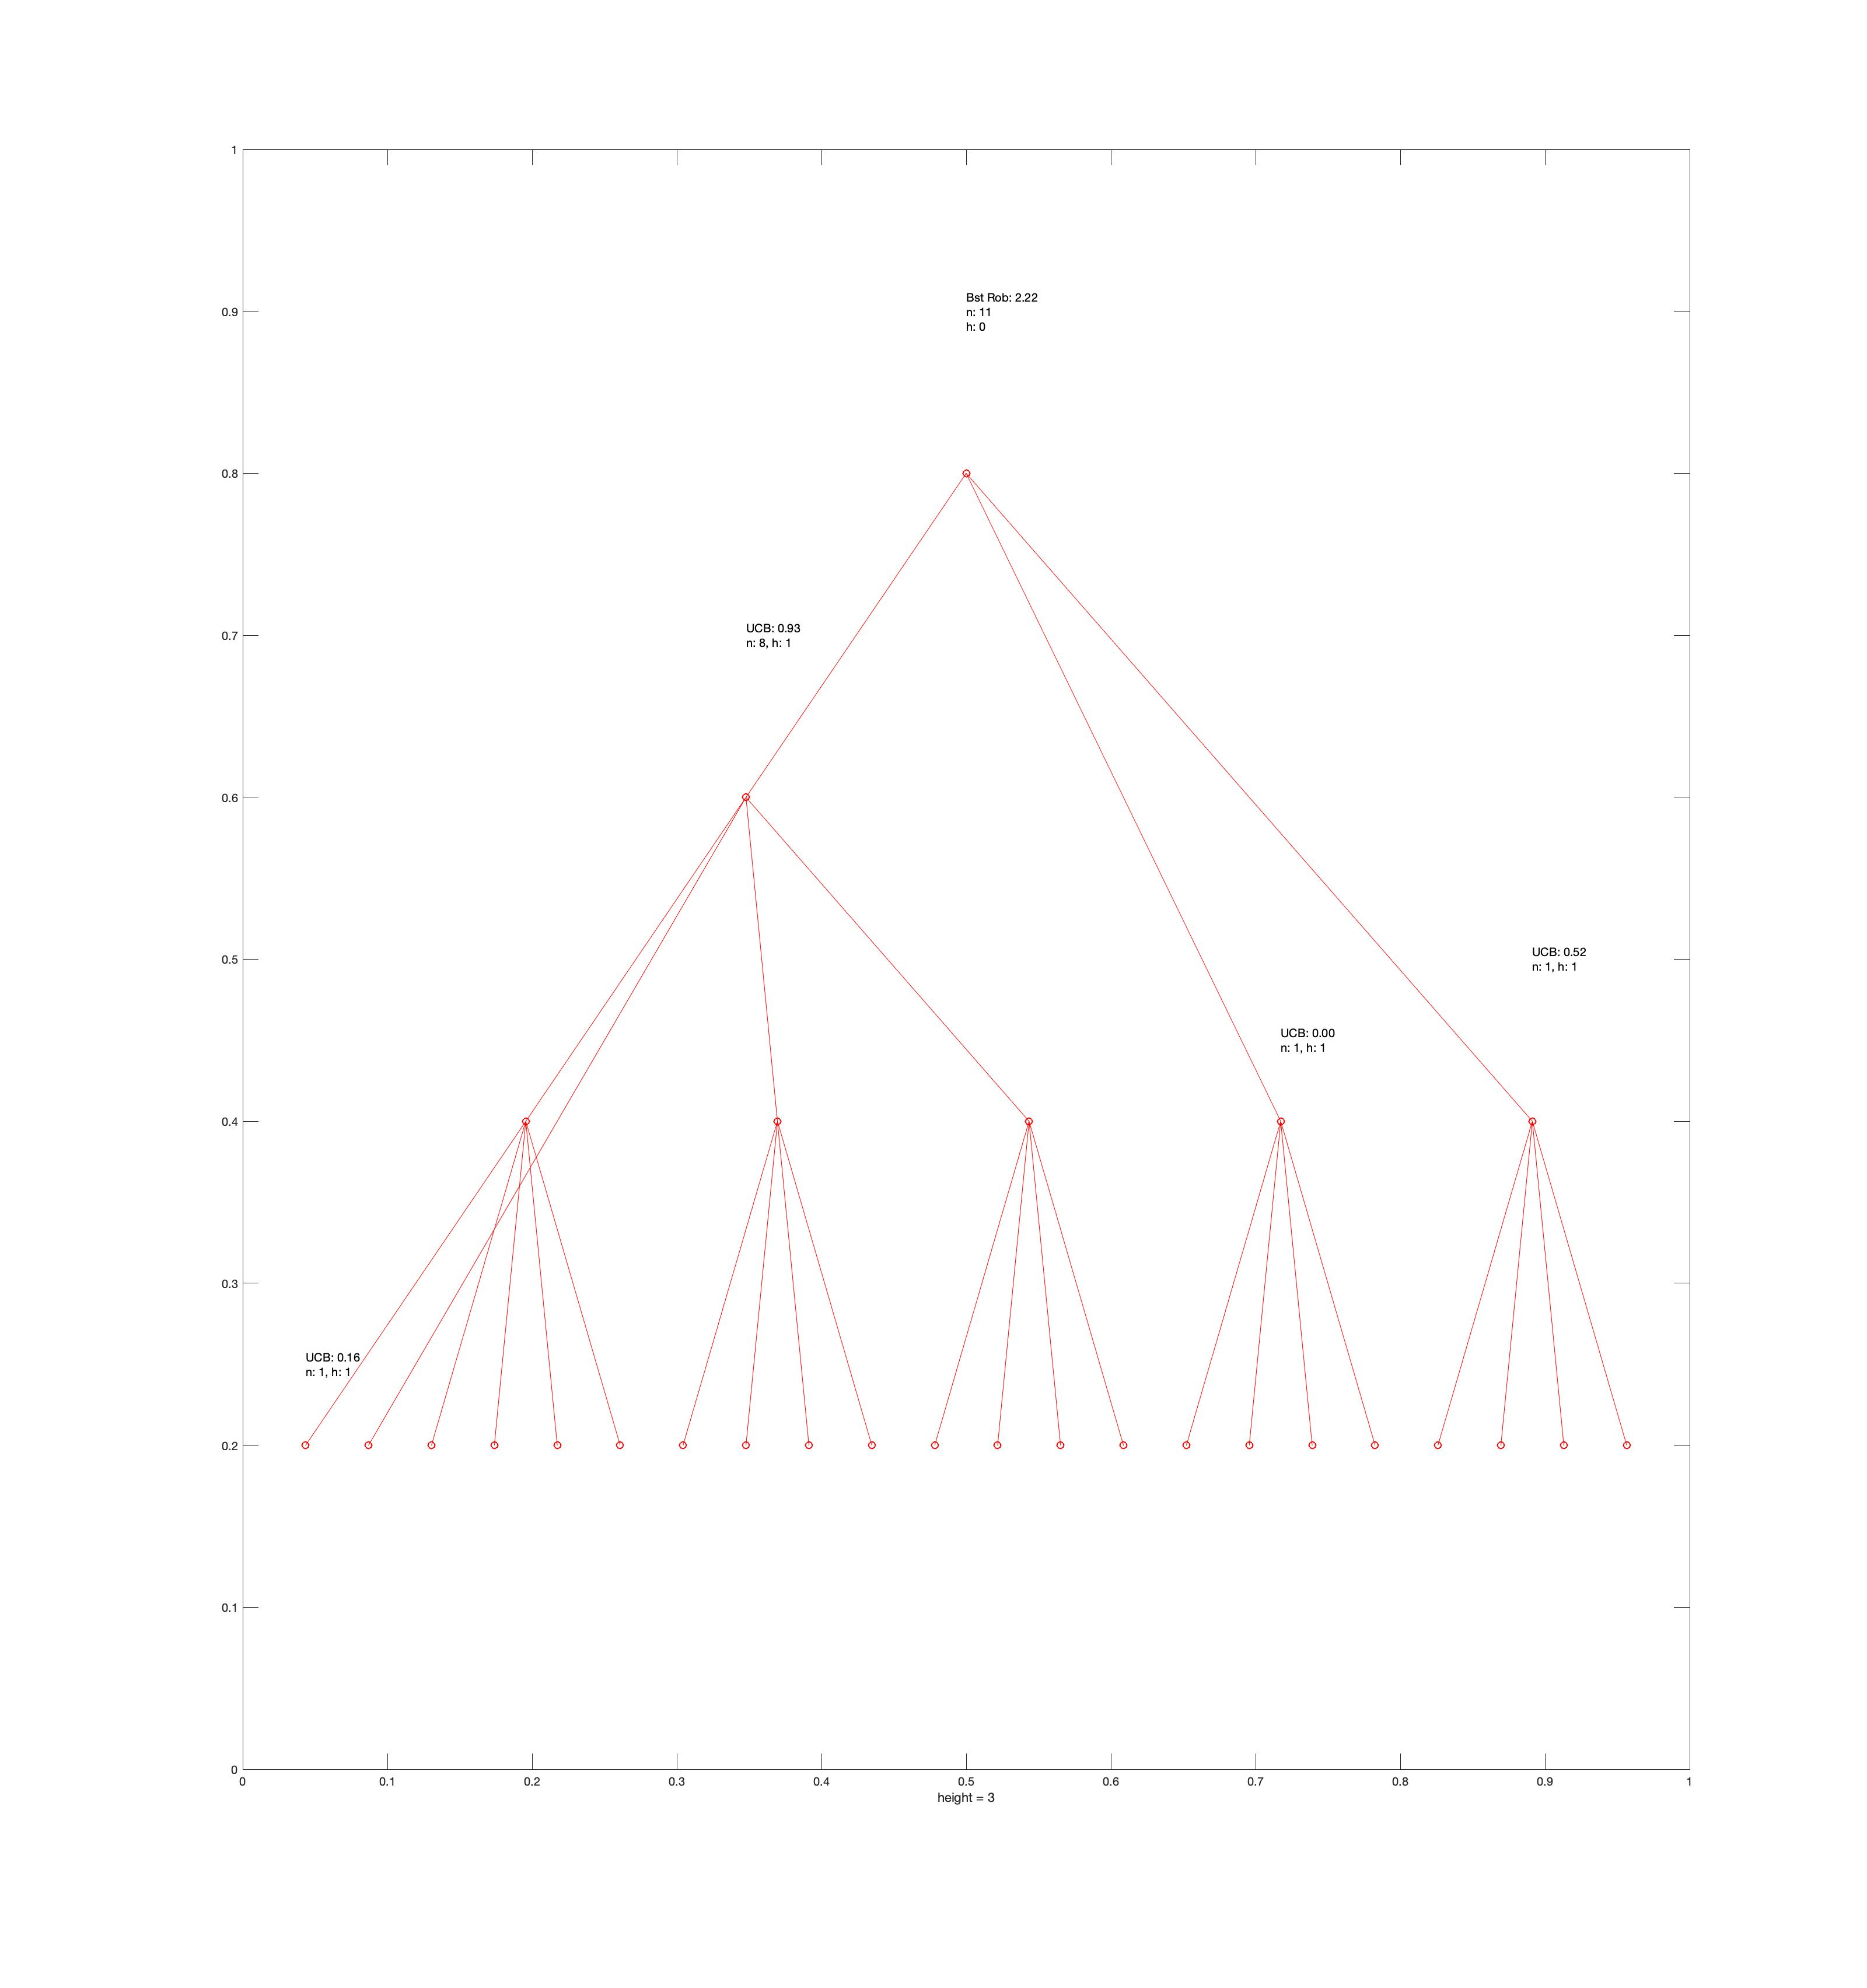
\includegraphics[width=0.4\linewidth]{img/c0.jpg}
%   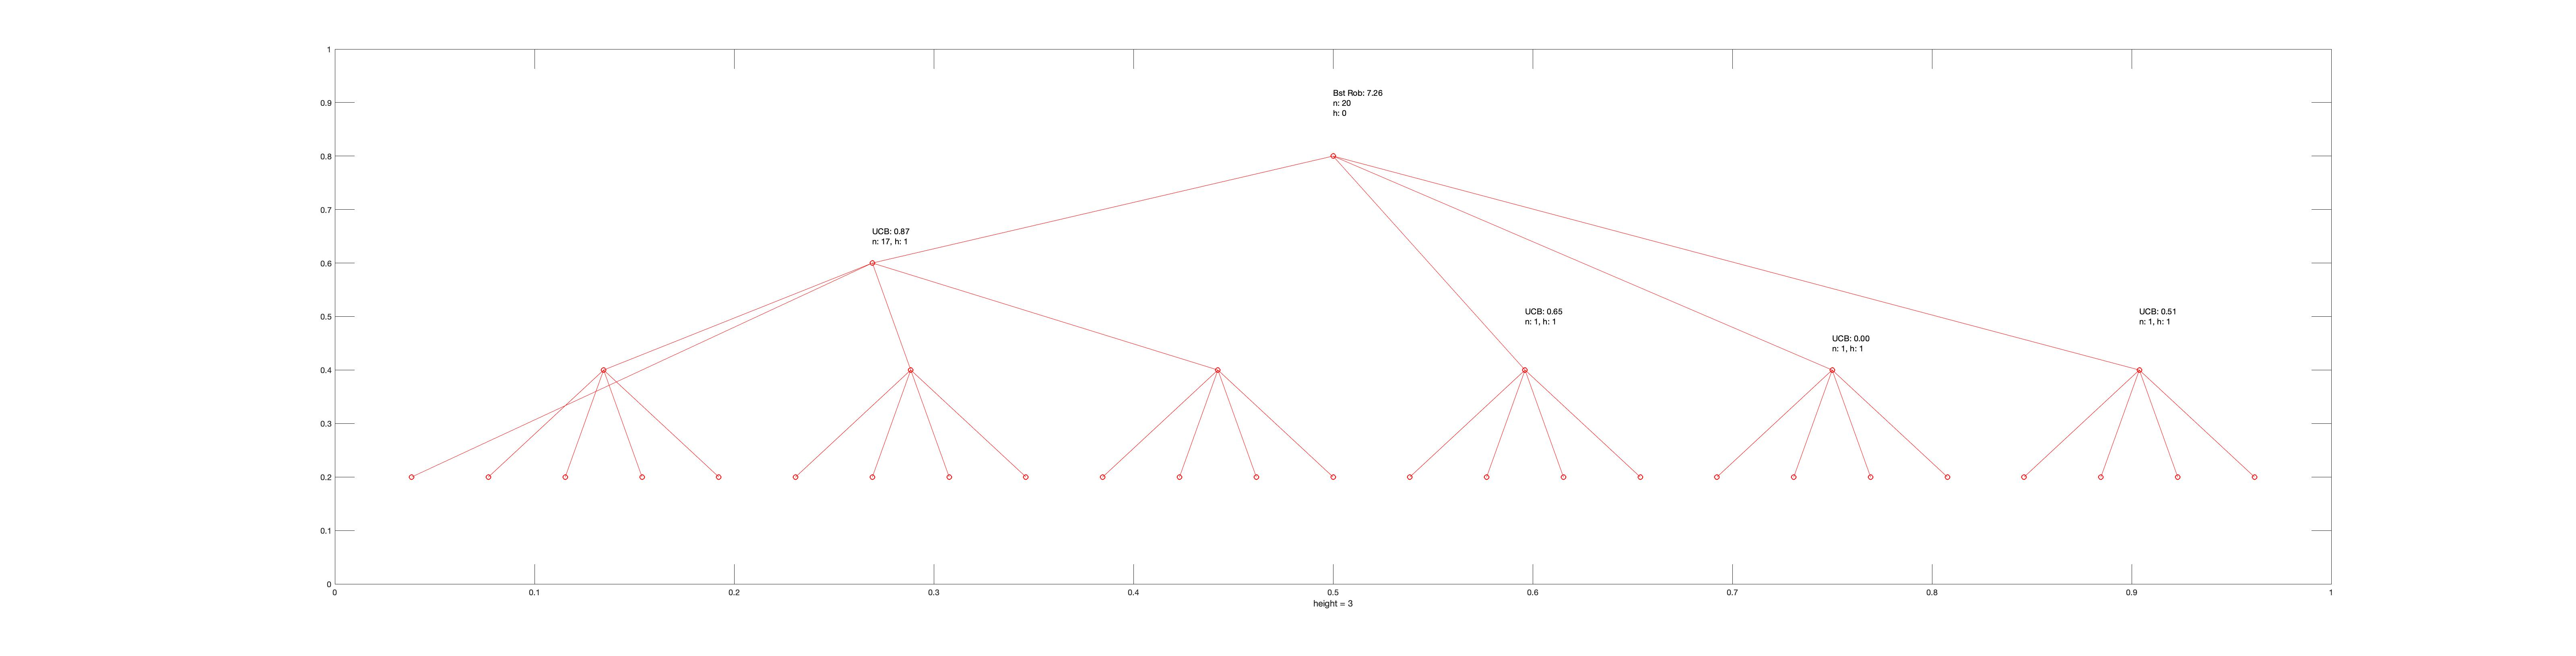
\includegraphics[width=\linewidth]{img/c00wide.jpg}
%   \caption{Favour exploitation ($C=0$).}
%   \label{fig:c0}
% \end{subfigure}\\
% \begin{subfigure}{\textwidth}
%   \centering
%   % 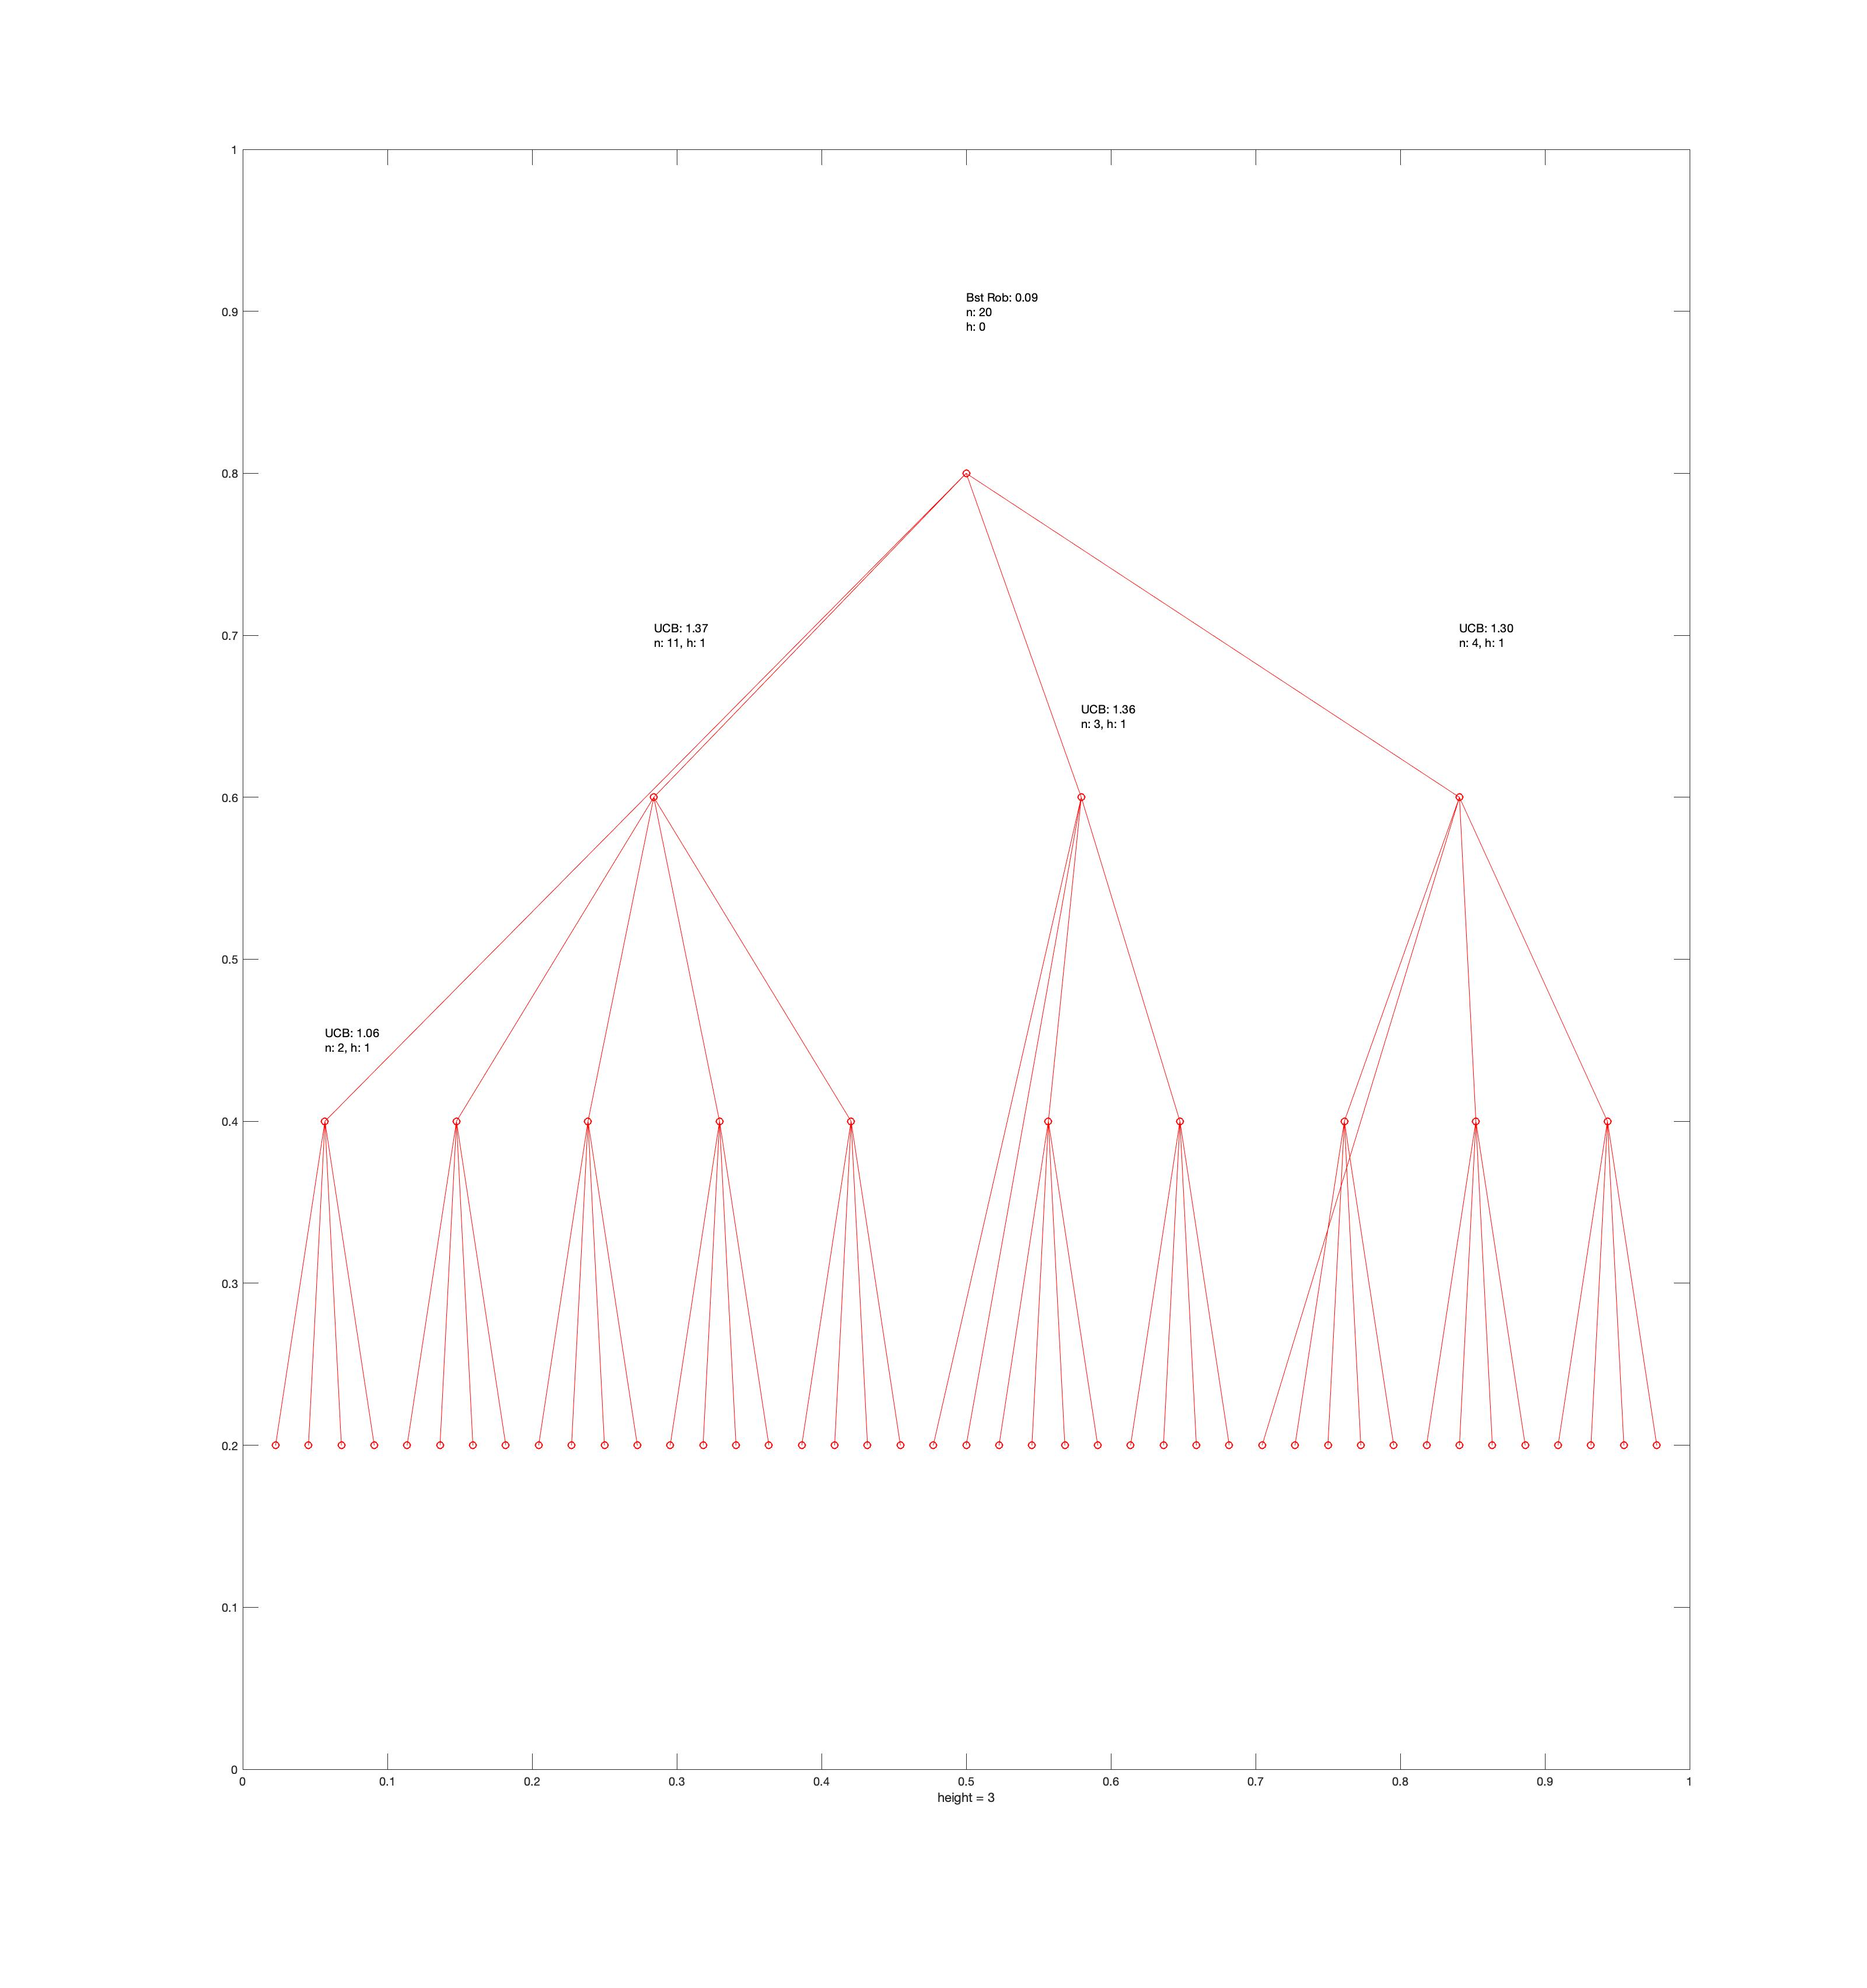
\includegraphics[width=0.4\linewidth]{img/c05.jpg}
  % 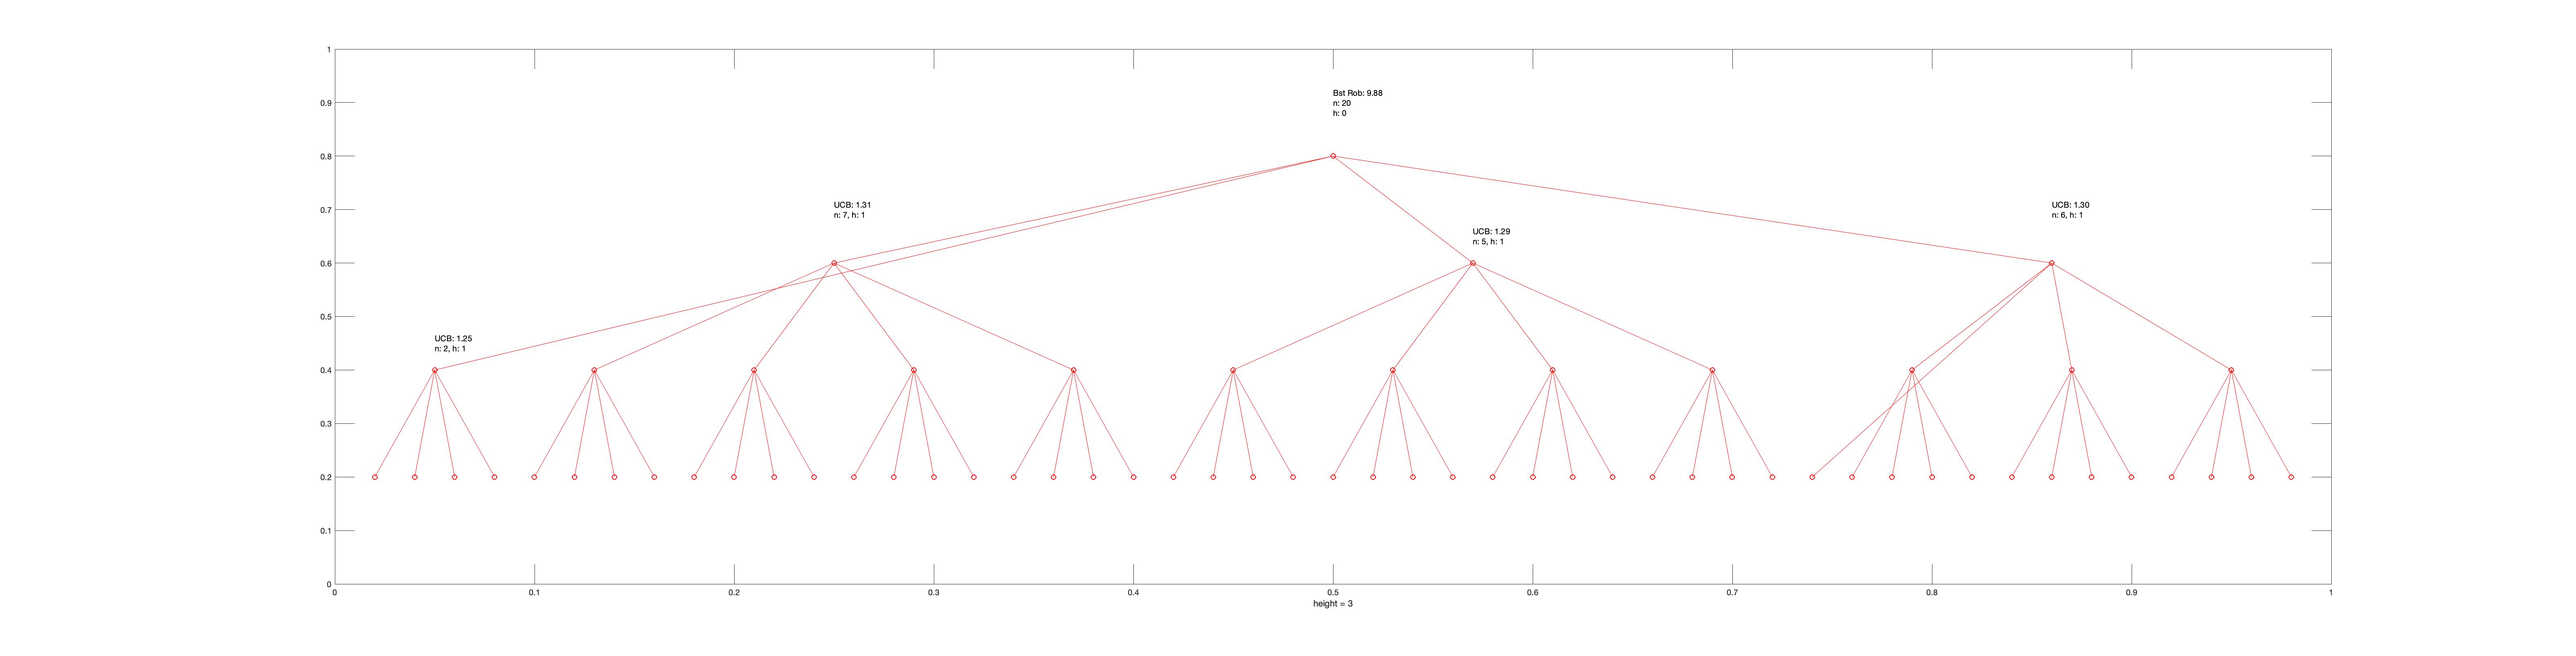
\includegraphics[width=\linewidth]{img/c05wide.jpg}
  % \caption{Balanced ($C=0.5$).}
  % \label{fig:c05}
% \end{subfigure}\\
% \begin{subfigure}{\textwidth}
  % \centering
  % % 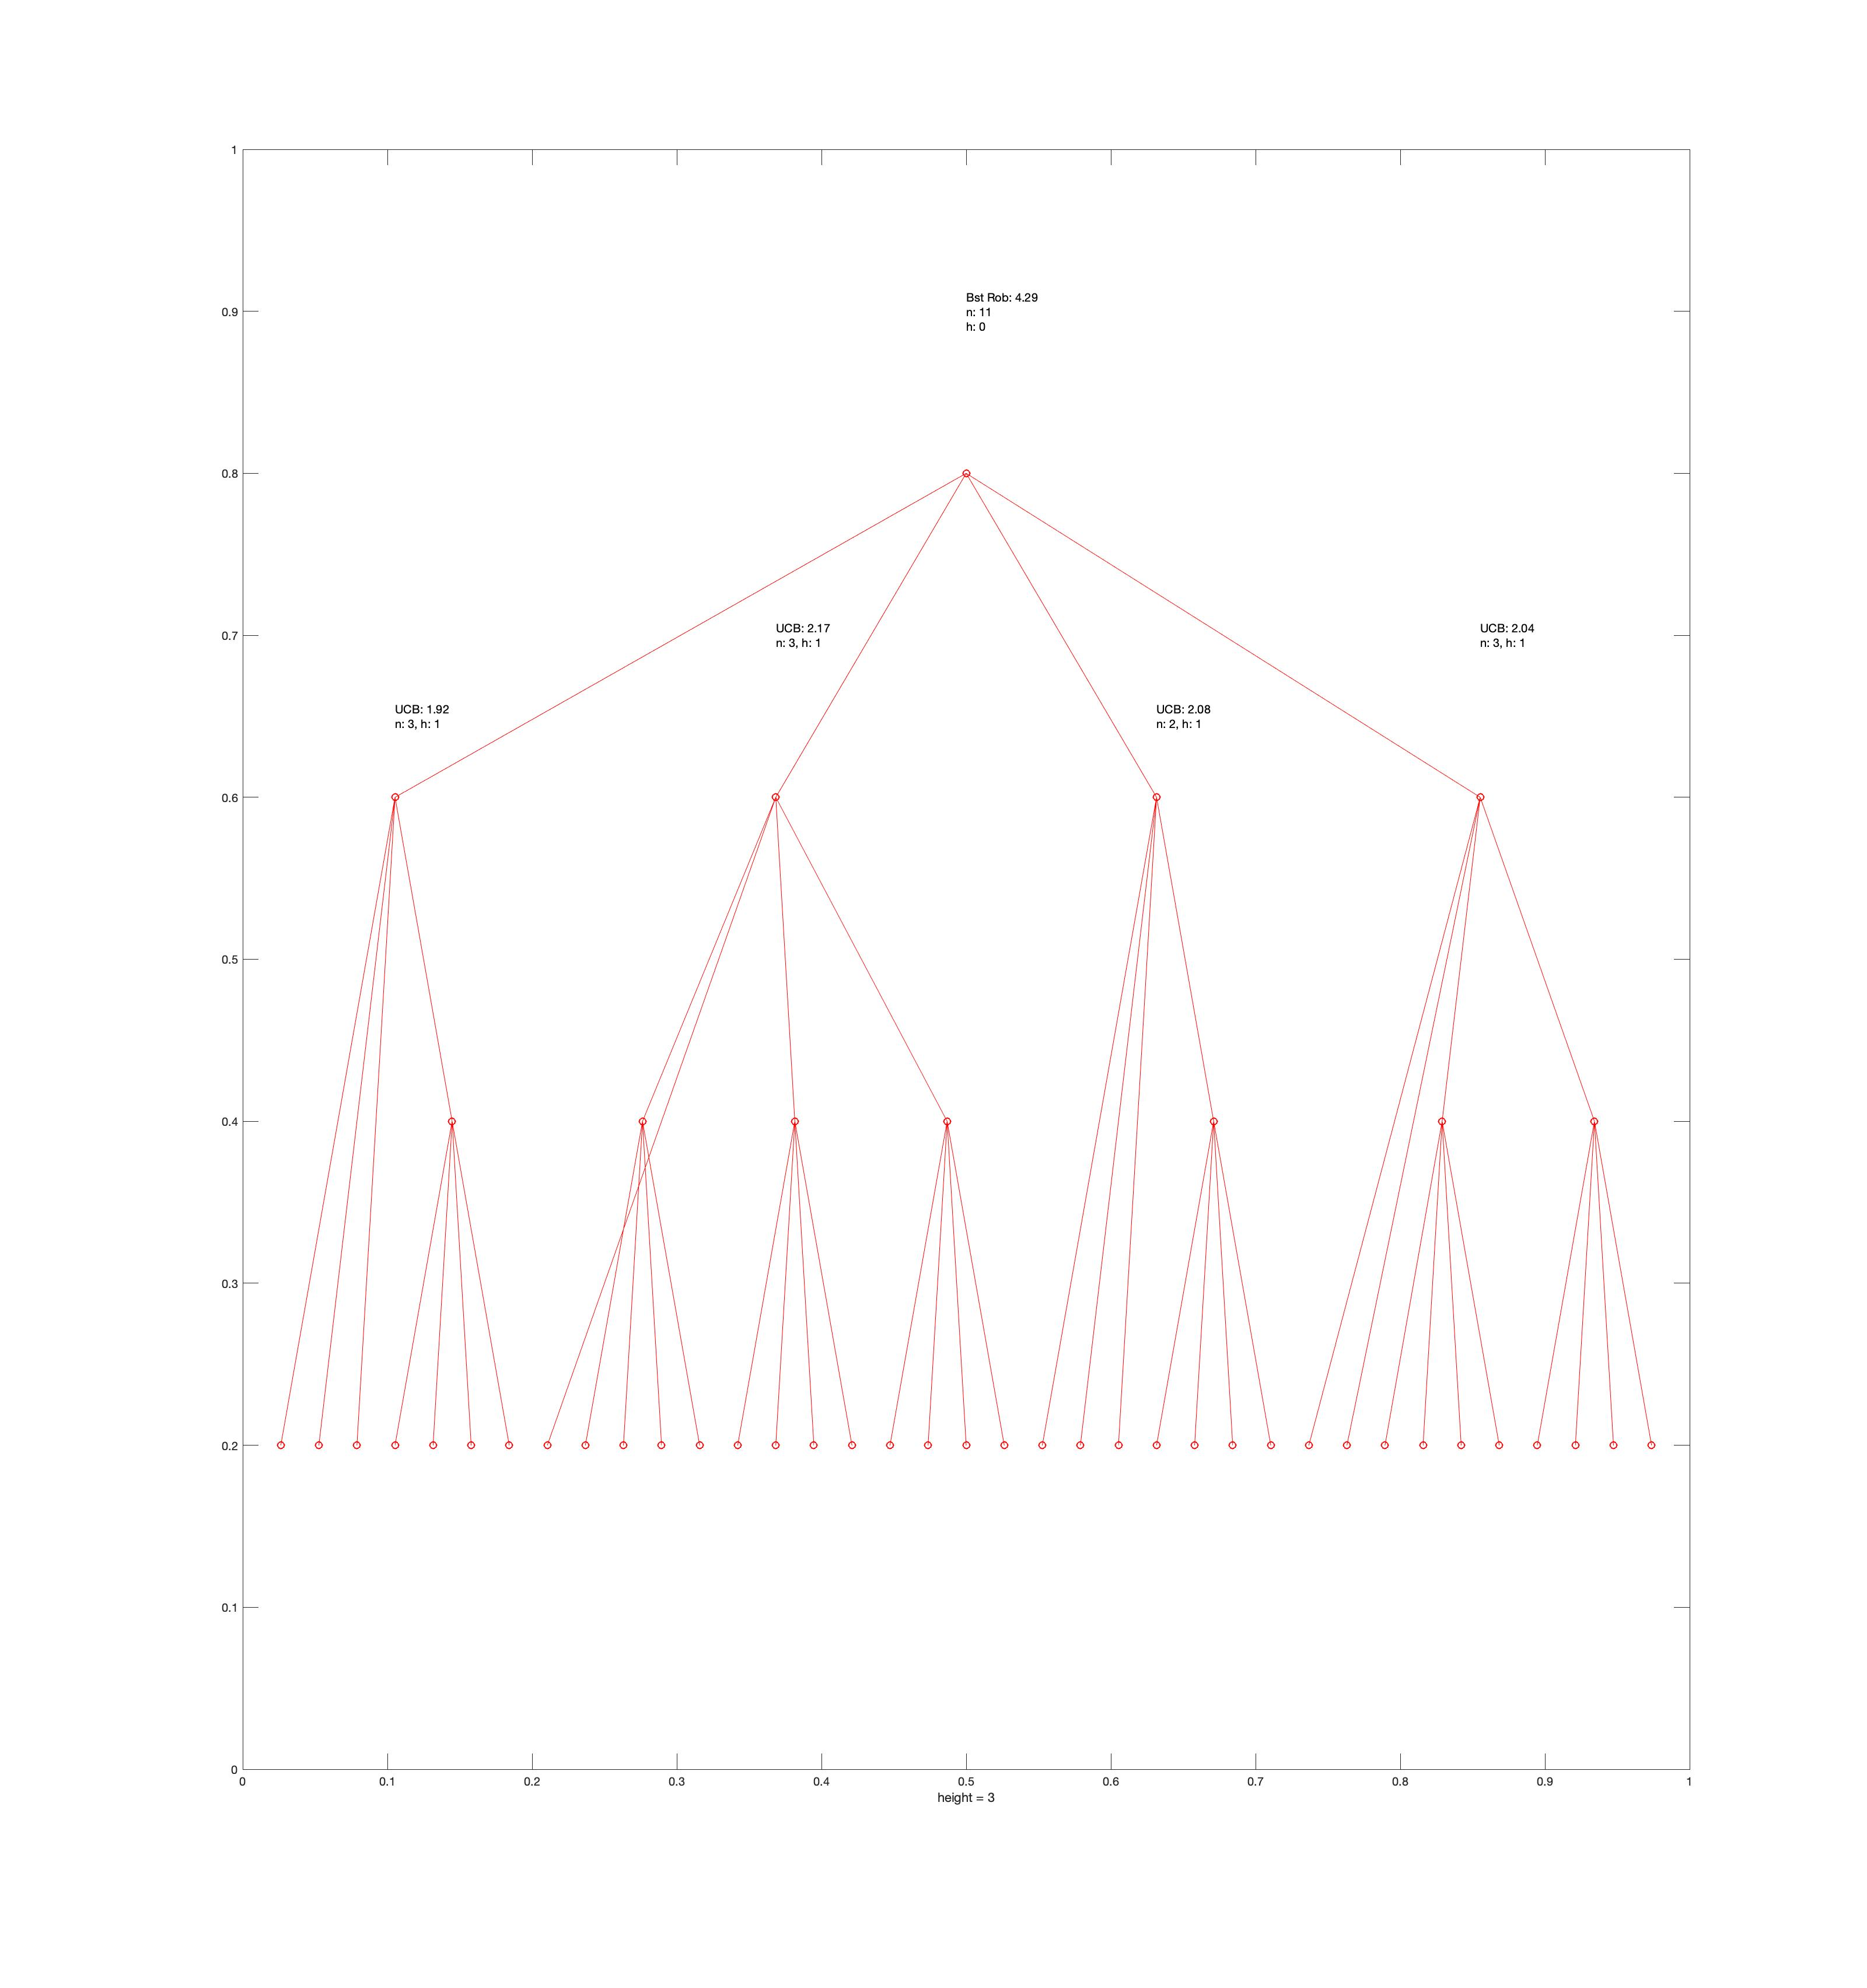
\includegraphics[width=0.4\linewidth]{img/c1.jpg}
  % 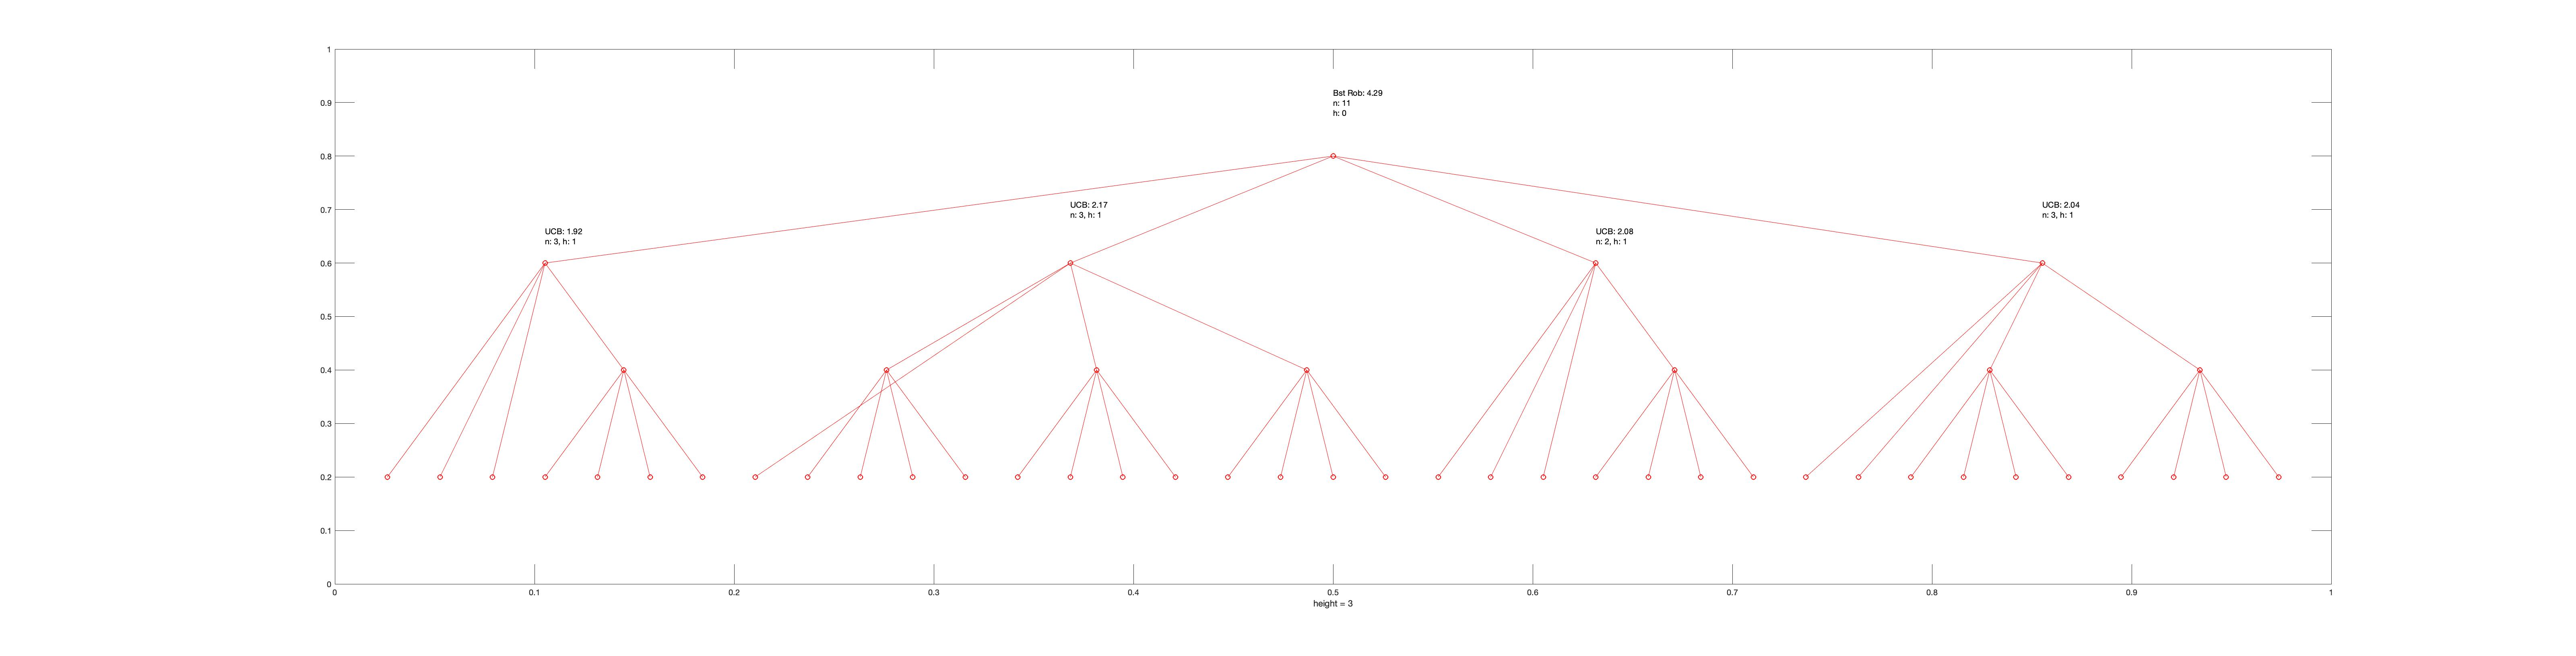
\includegraphics[width=\linewidth]{img/c10wide.jpg}
  % \caption{Favour exploration ($C=1$).}
  % \label{fig:c1}
% \end{subfigure}
% \caption{Different MCTS tree varying parameter $C$.}
% \label{fig:C}
% \end{figure}
%%%%%%%%%%%%%%%% MAYBE THIS IS BETTER?^^


% \begin{figure}
% \begin{subfigure}{.33\textwidth}
%   \centering
%   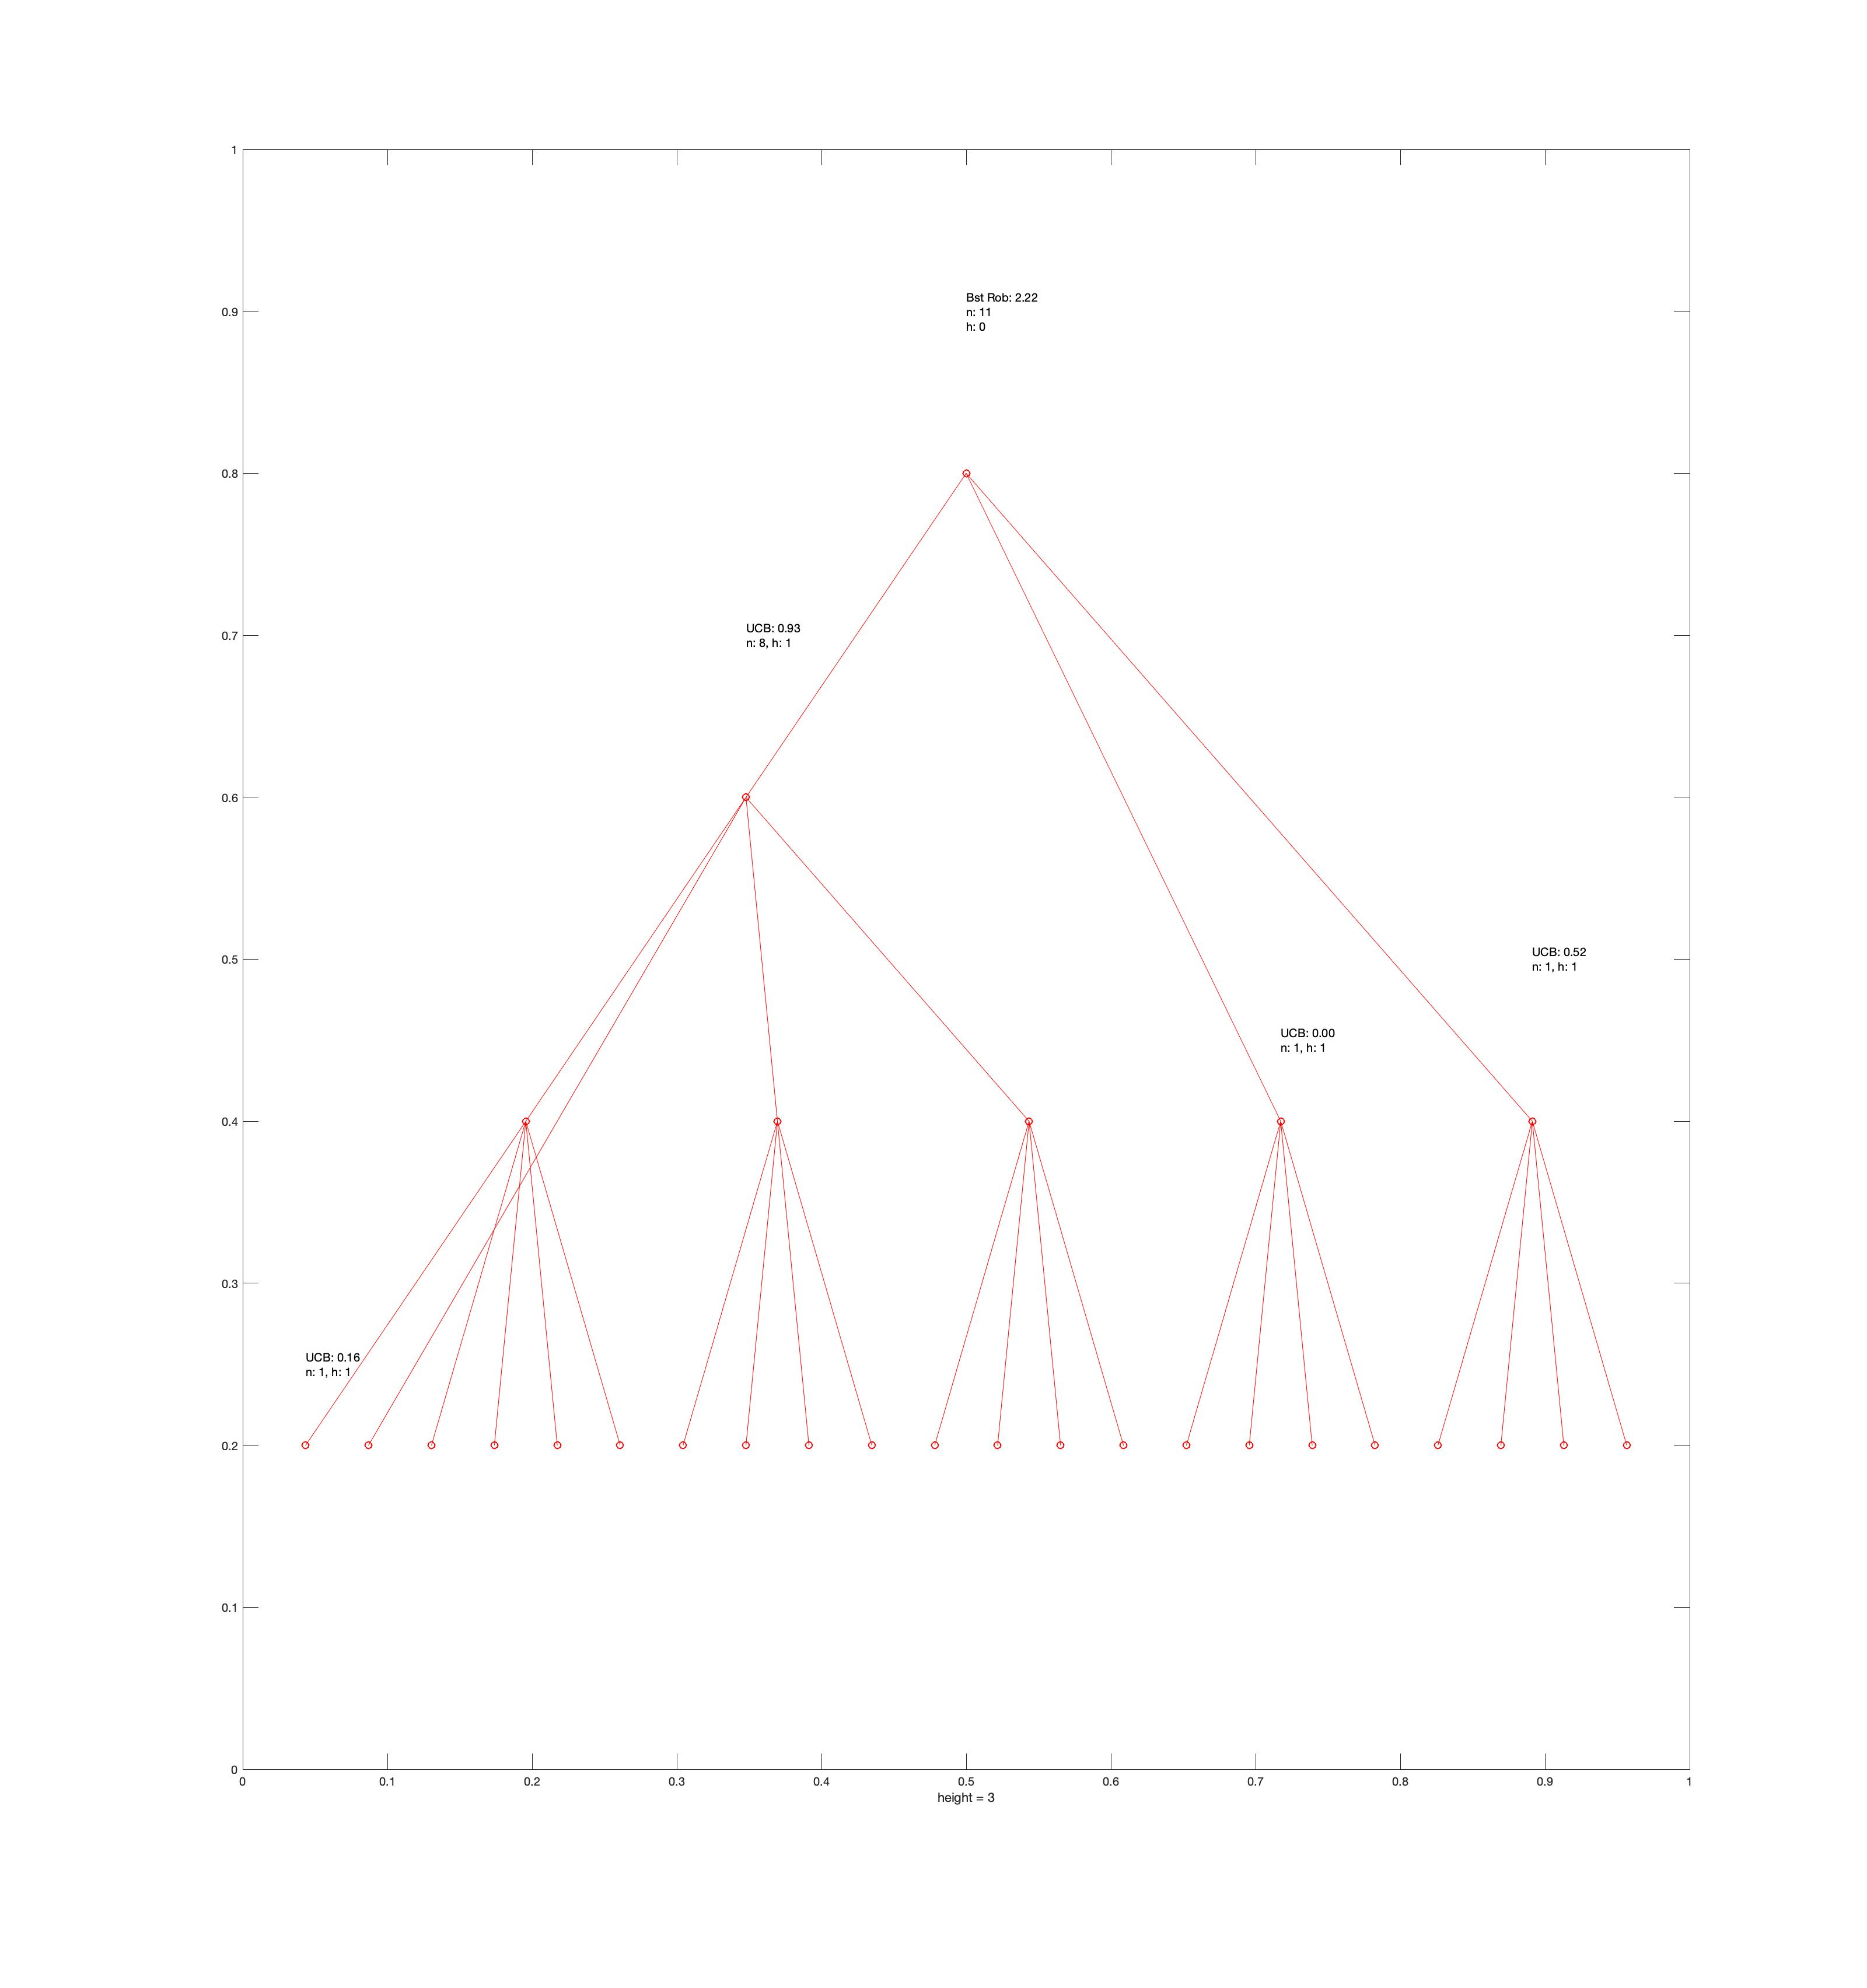
\includegraphics[width=\linewidth]{img/c0.jpg}
%   \caption{Favour exploitation ($C=0$).}
%   \label{fig:c0}
% \end{subfigure}%
% \begin{subfigure}{.33\textwidth}
%   \centering
%   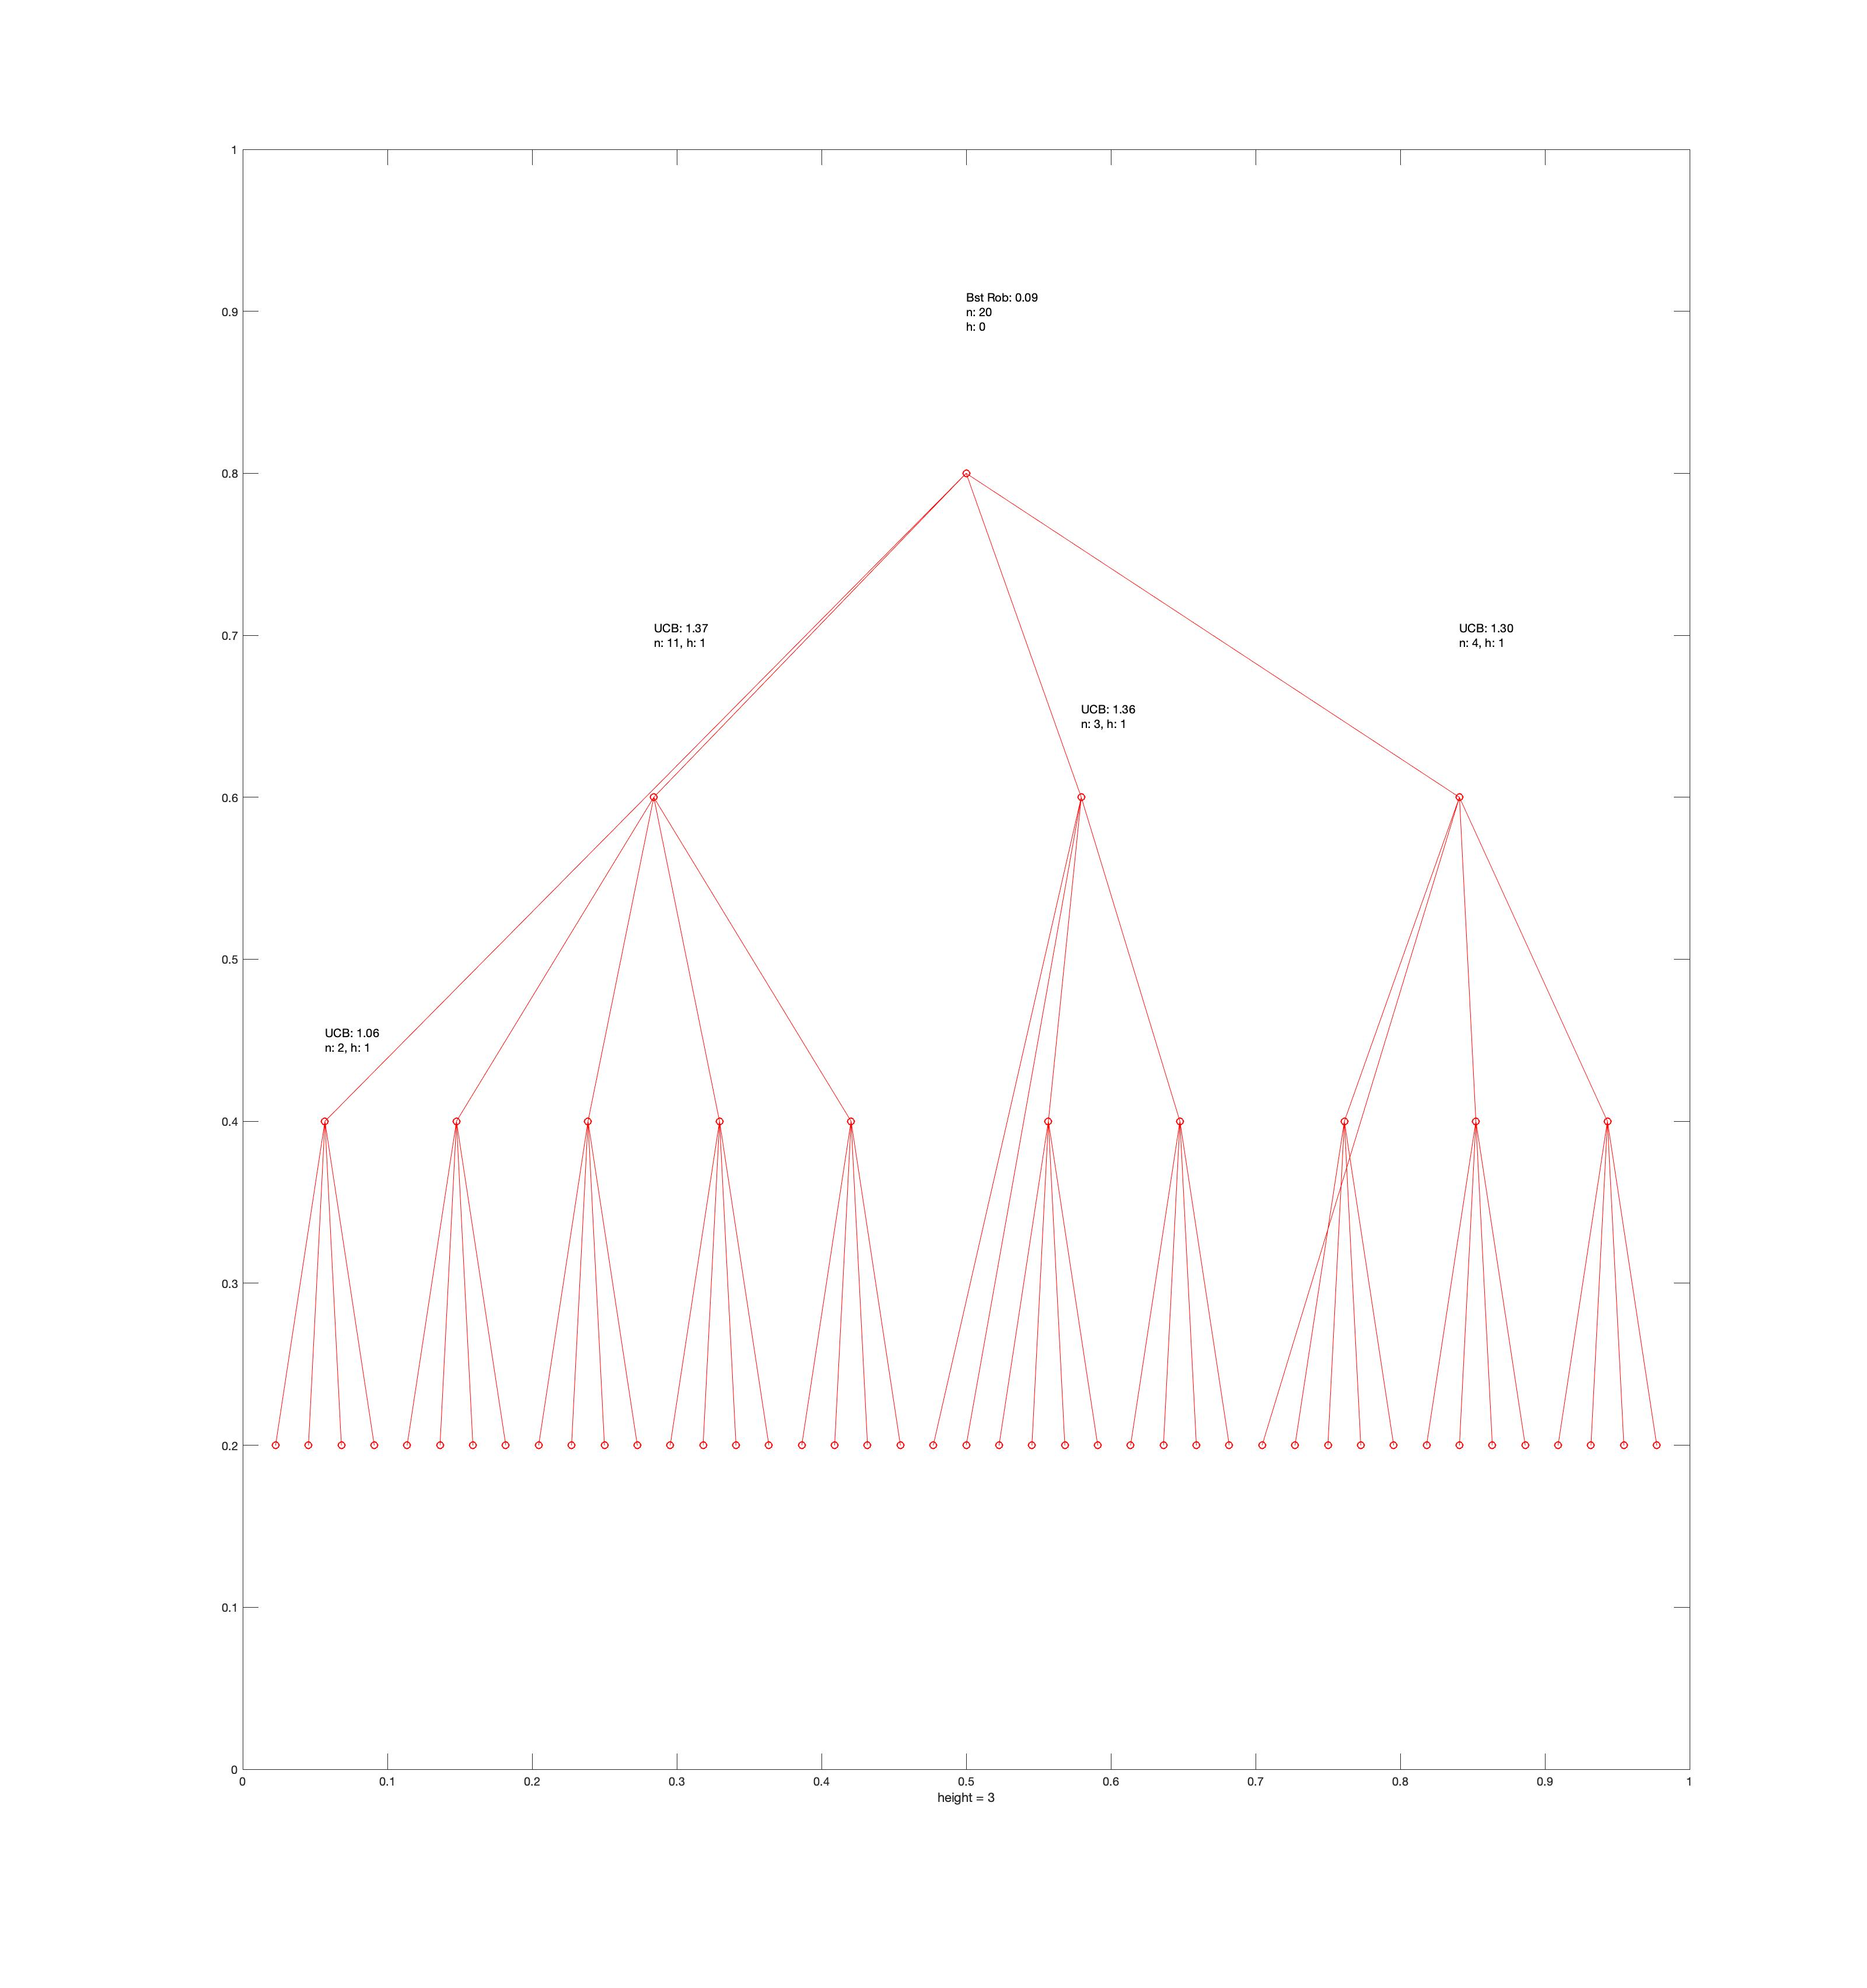
\includegraphics[width=\linewidth]{img/c05.jpg}
%   \caption{Balanced ($C=0.5$).}
%   \label{fig:c05}
% \end{subfigure}%
% \begin{subfigure}{.33\textwidth}
%   \centering
%   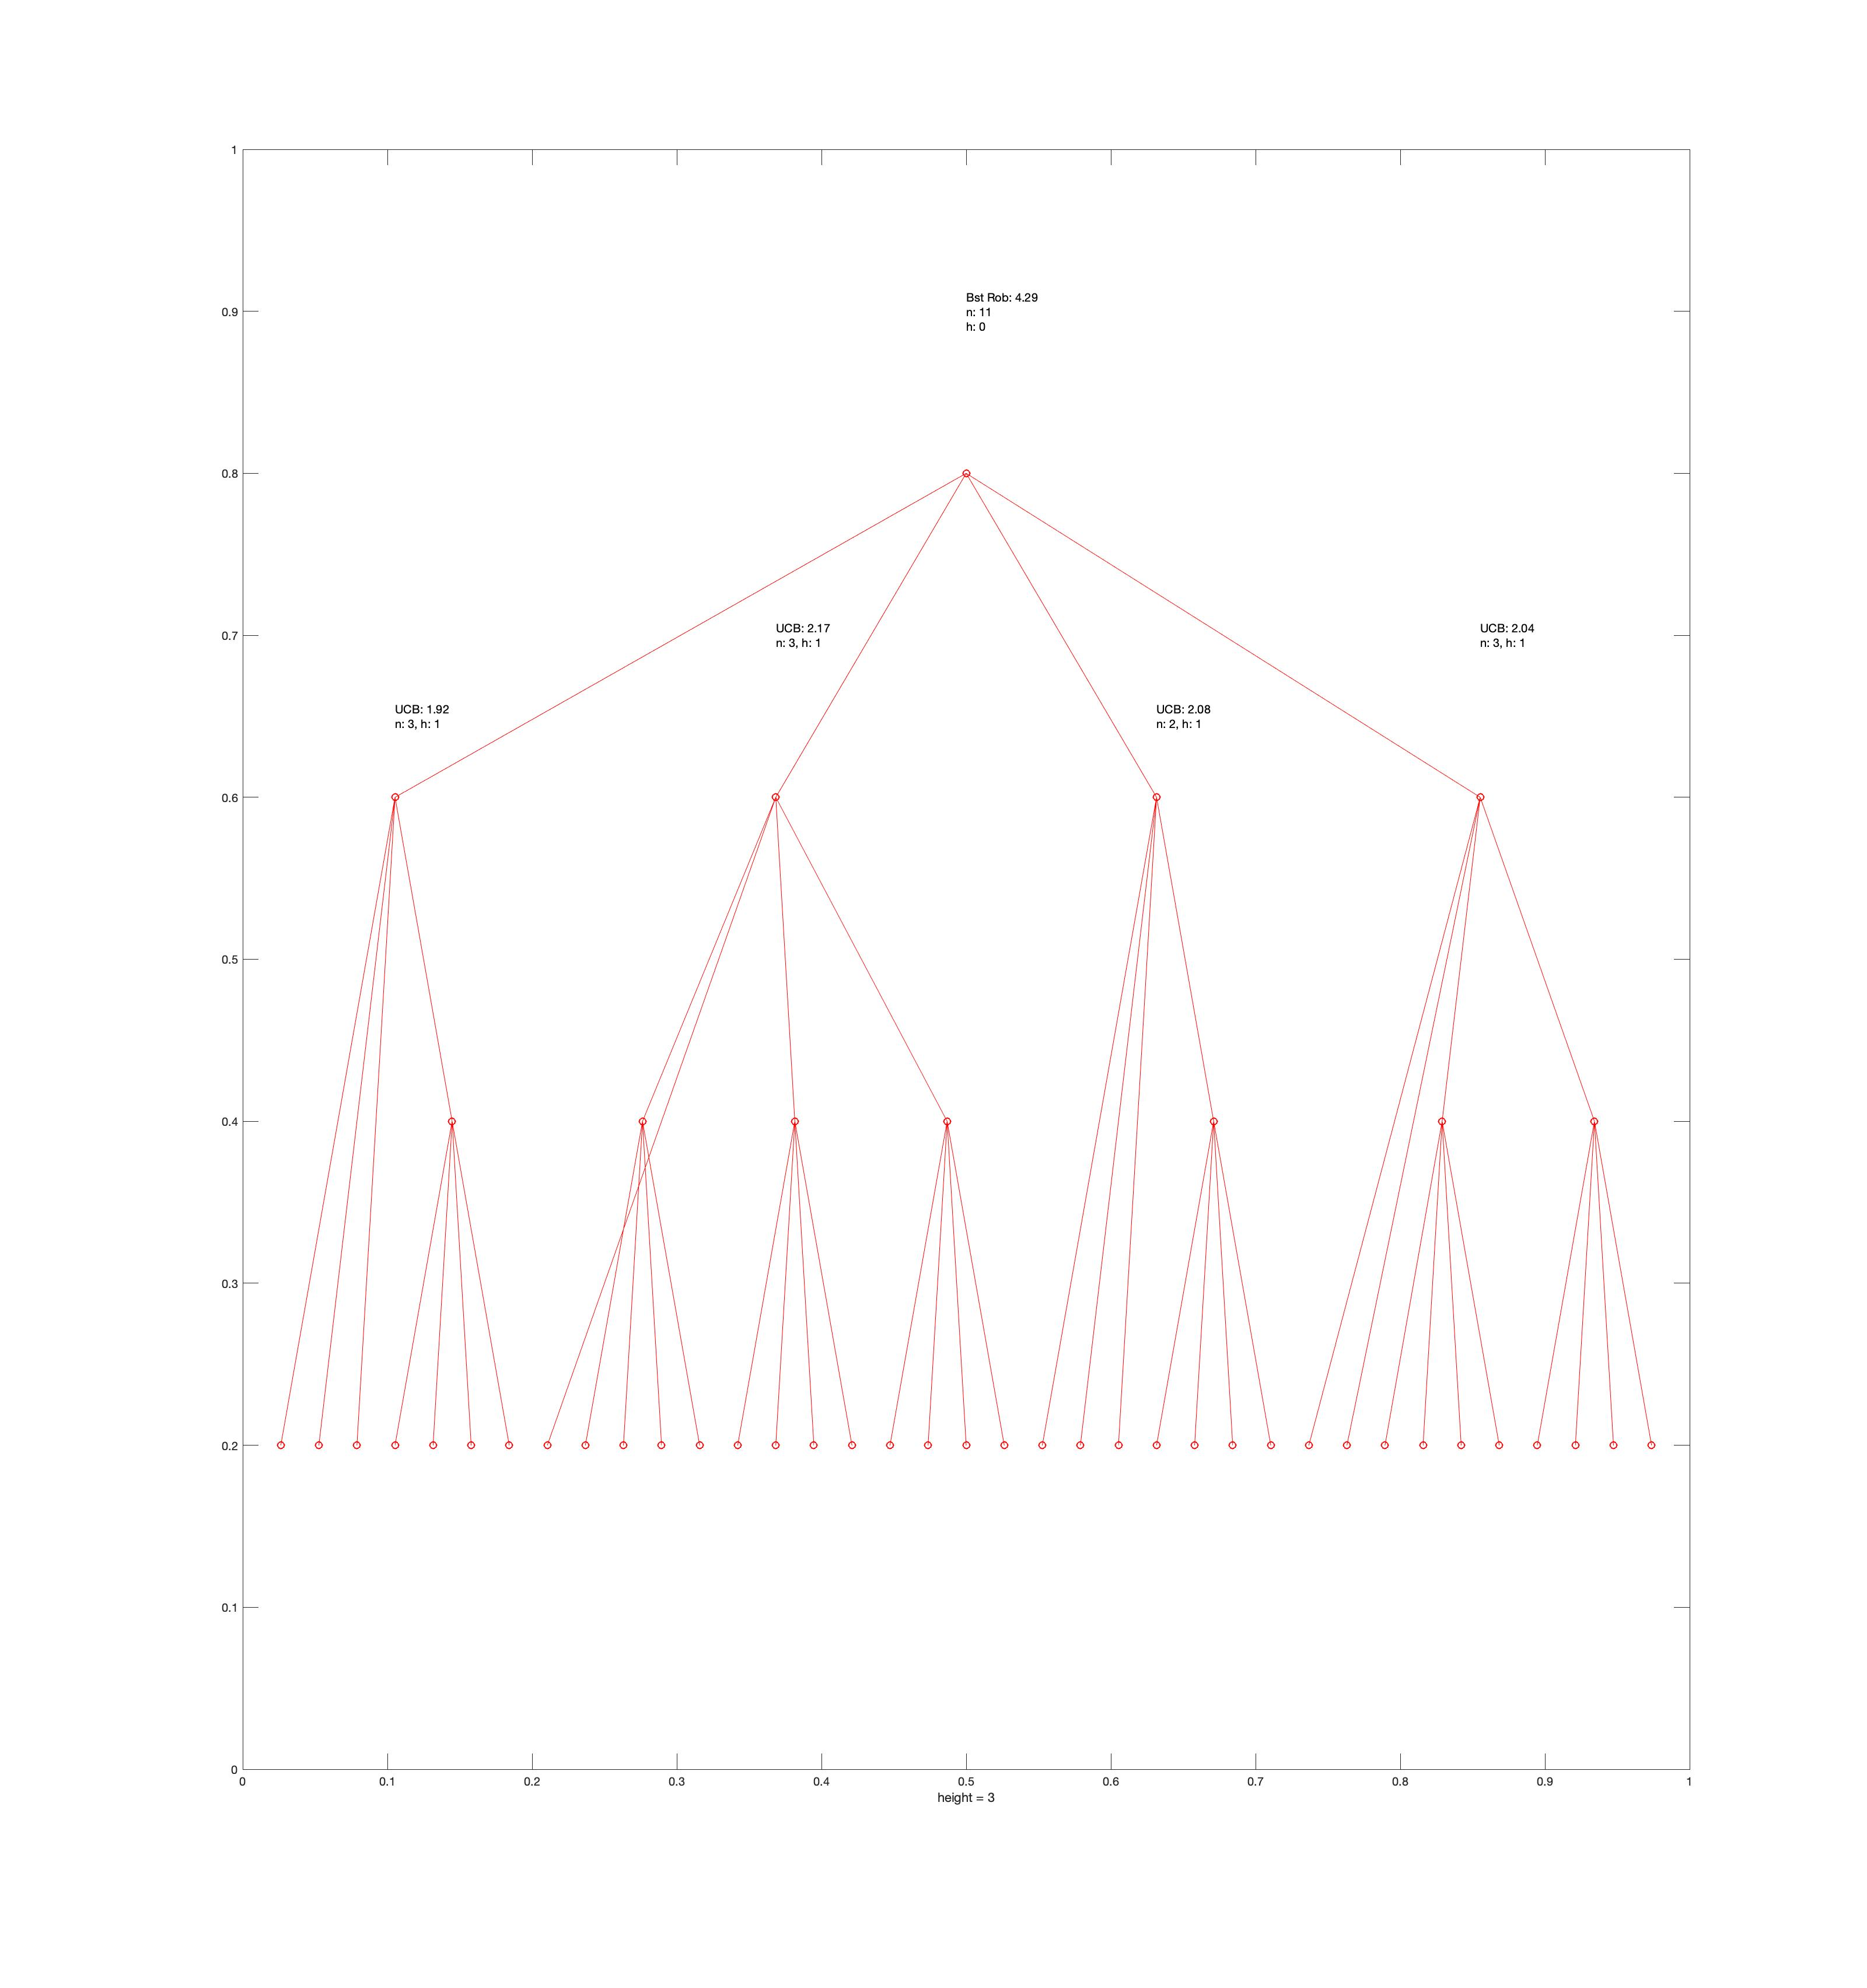
\includegraphics[width=\linewidth]{img/c1.jpg}
%   \caption{Favour exploration ($C=1$).}
%   \label{fig:c1}
% \end{subfigure}
% \caption{Different MCTS tree varying parameter $C$.}
% \label{fig:C}
% \end{figure}

\begin{figure}
  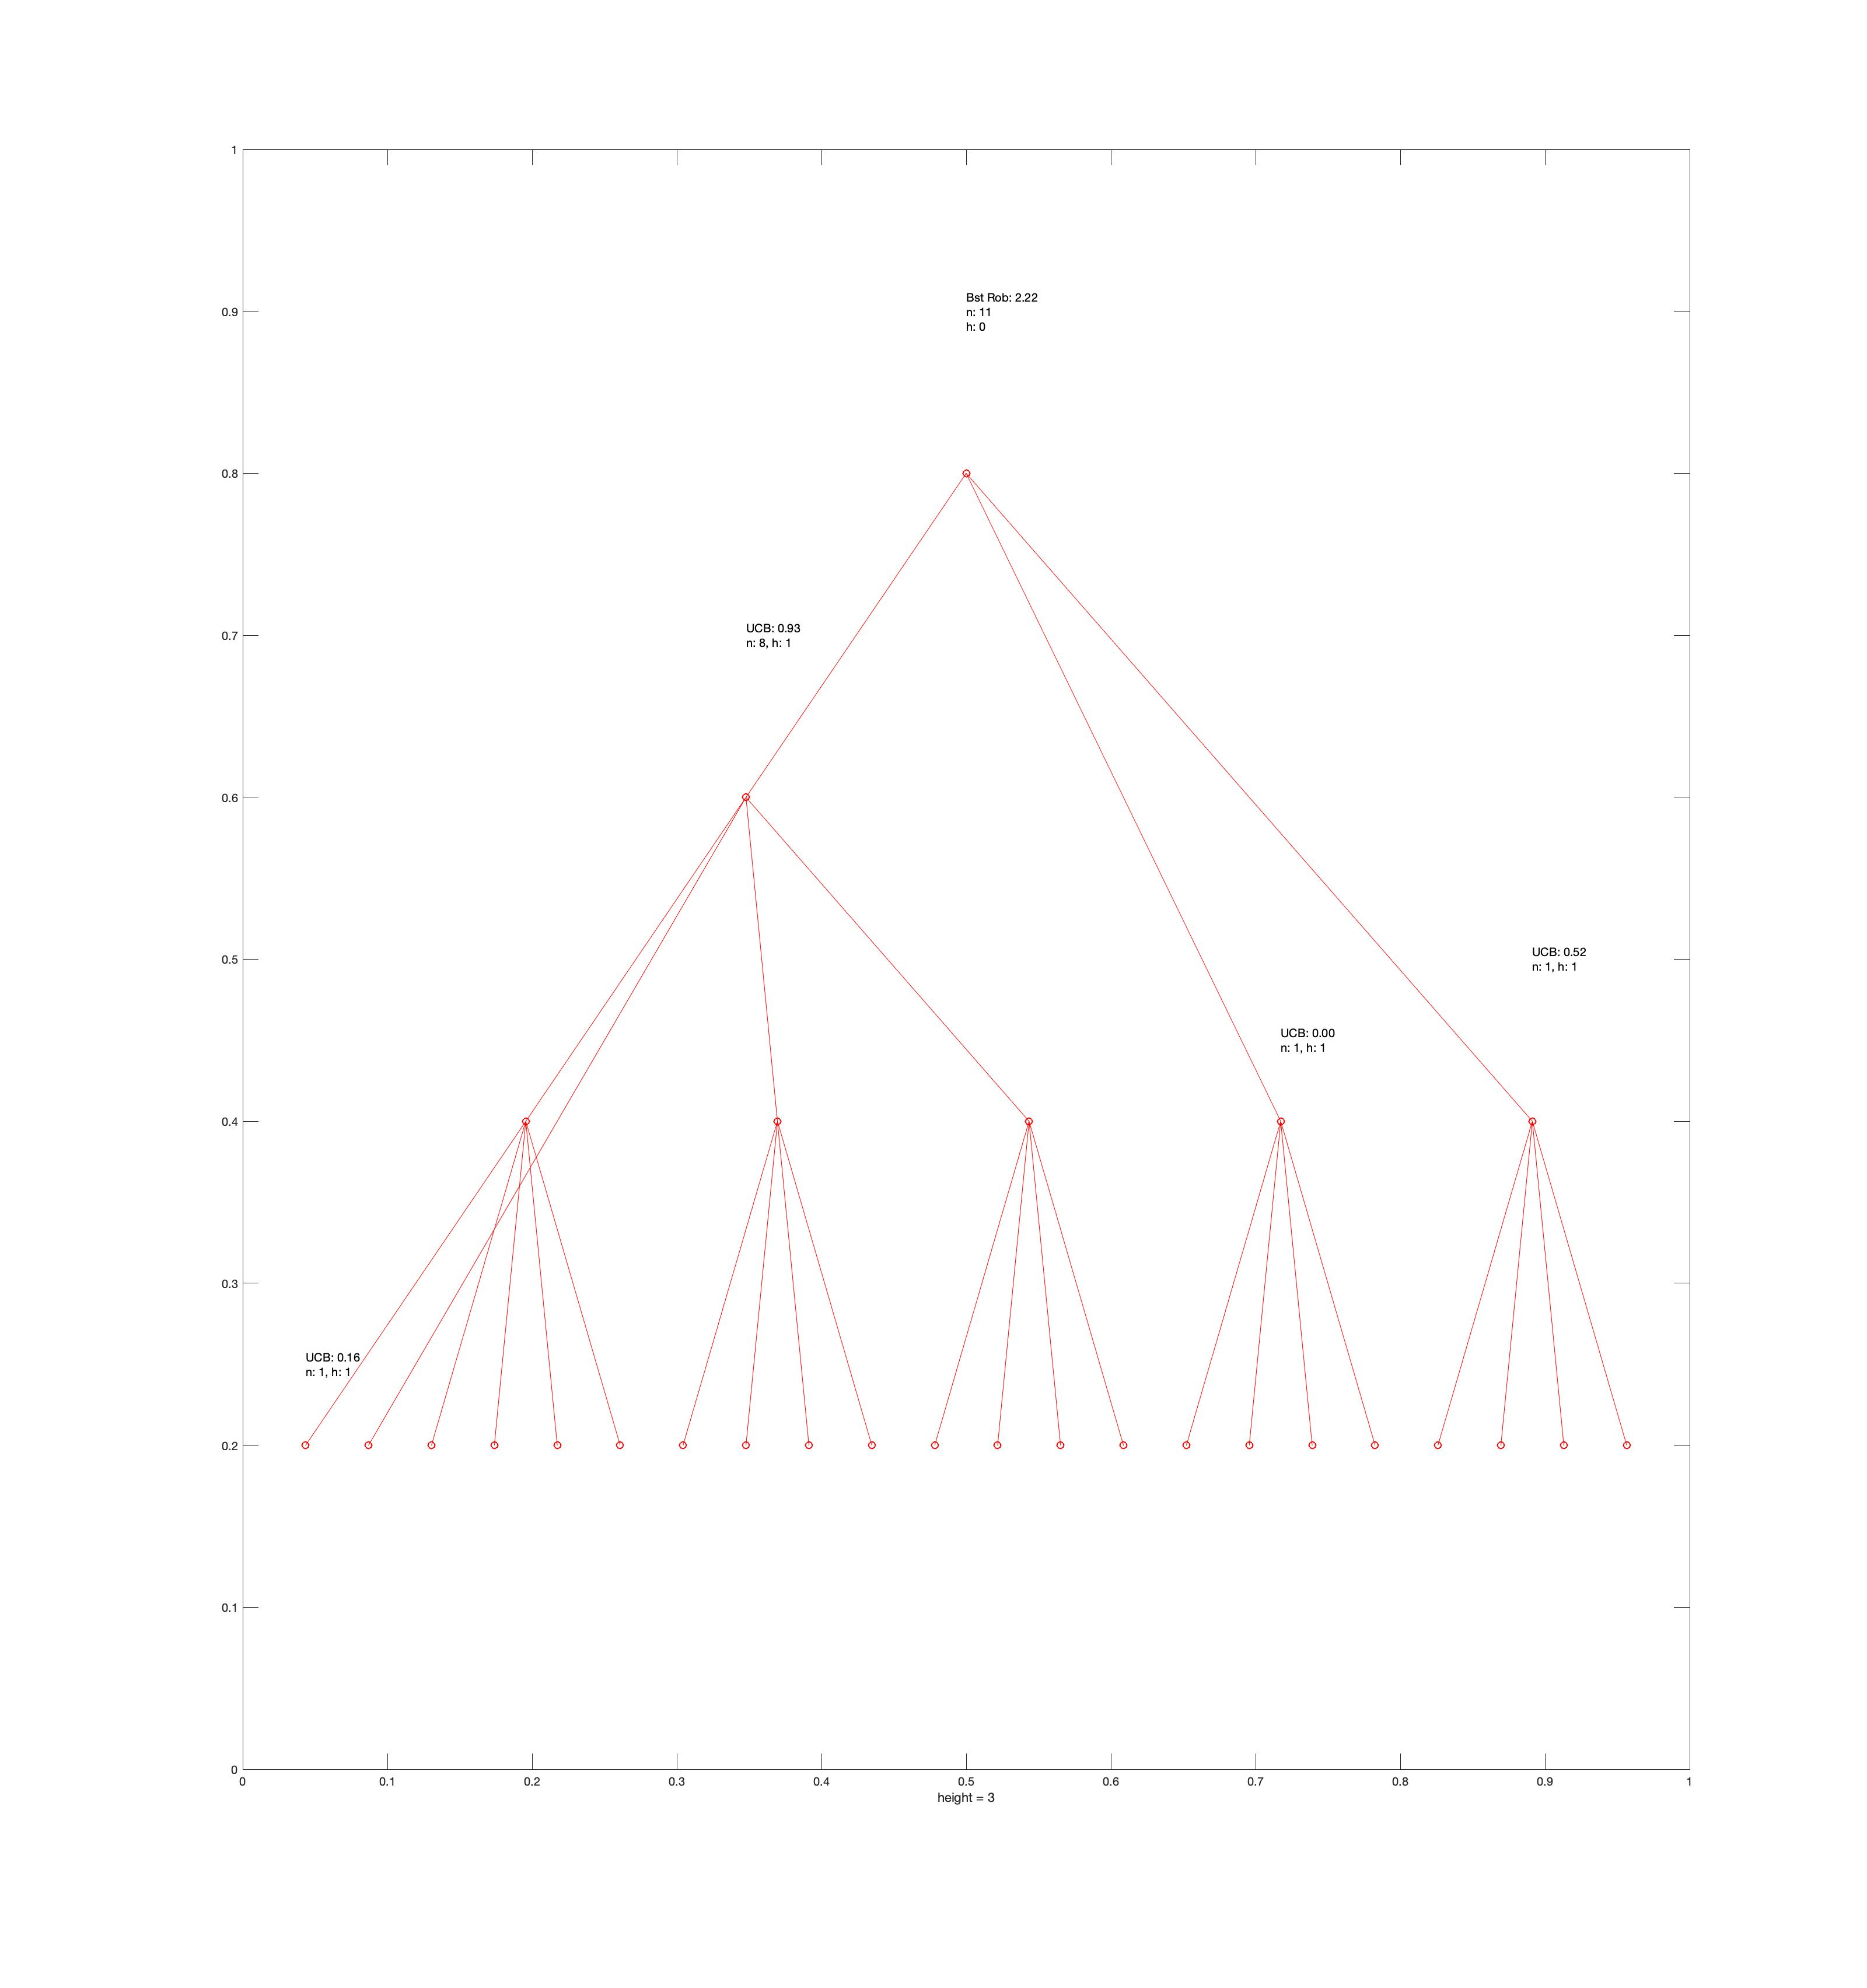
\includegraphics[width=\linewidth]{img/c0.jpg}
  \caption{MCTS: Favour exploitation ($C=0$).}
  \label{fig:c0}
\end{figure}
\begin{figure}
  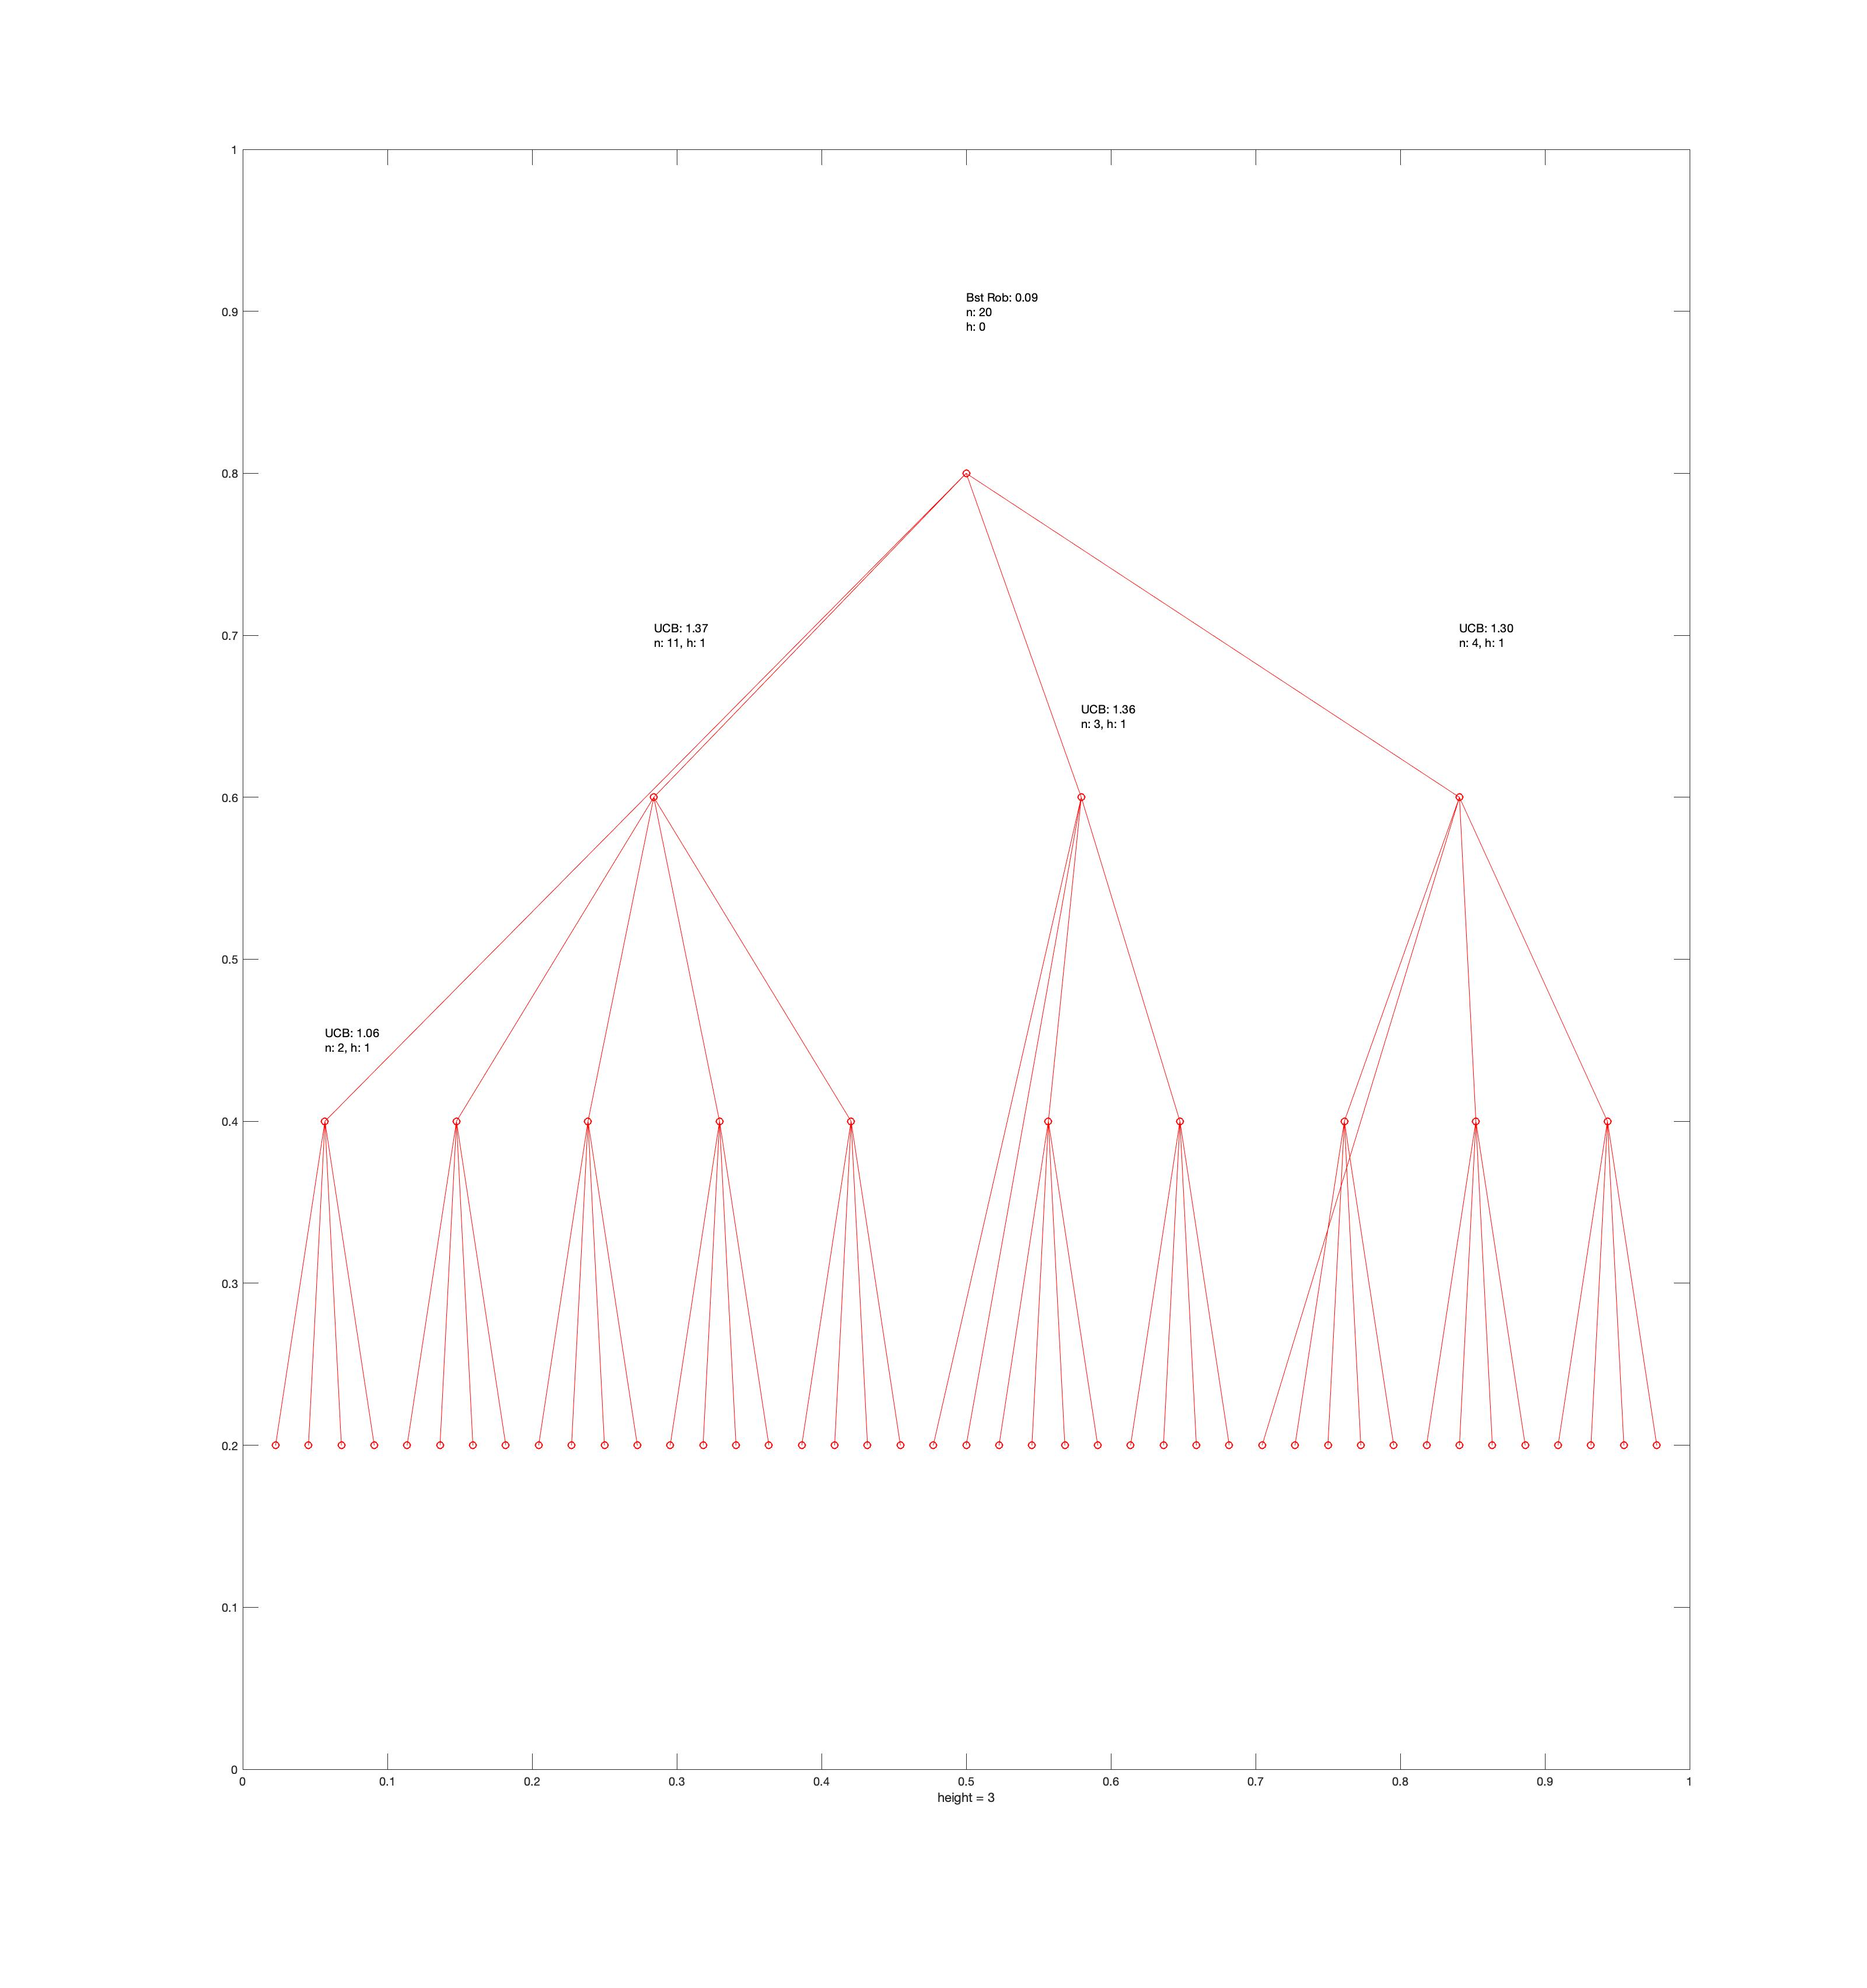
\includegraphics[width=\linewidth]{img/c05.jpg}
  \caption{MCTS: Balanced ($C=0.5$).}
  \label{fig:c05}
\end{figure}
\begin{figure}
  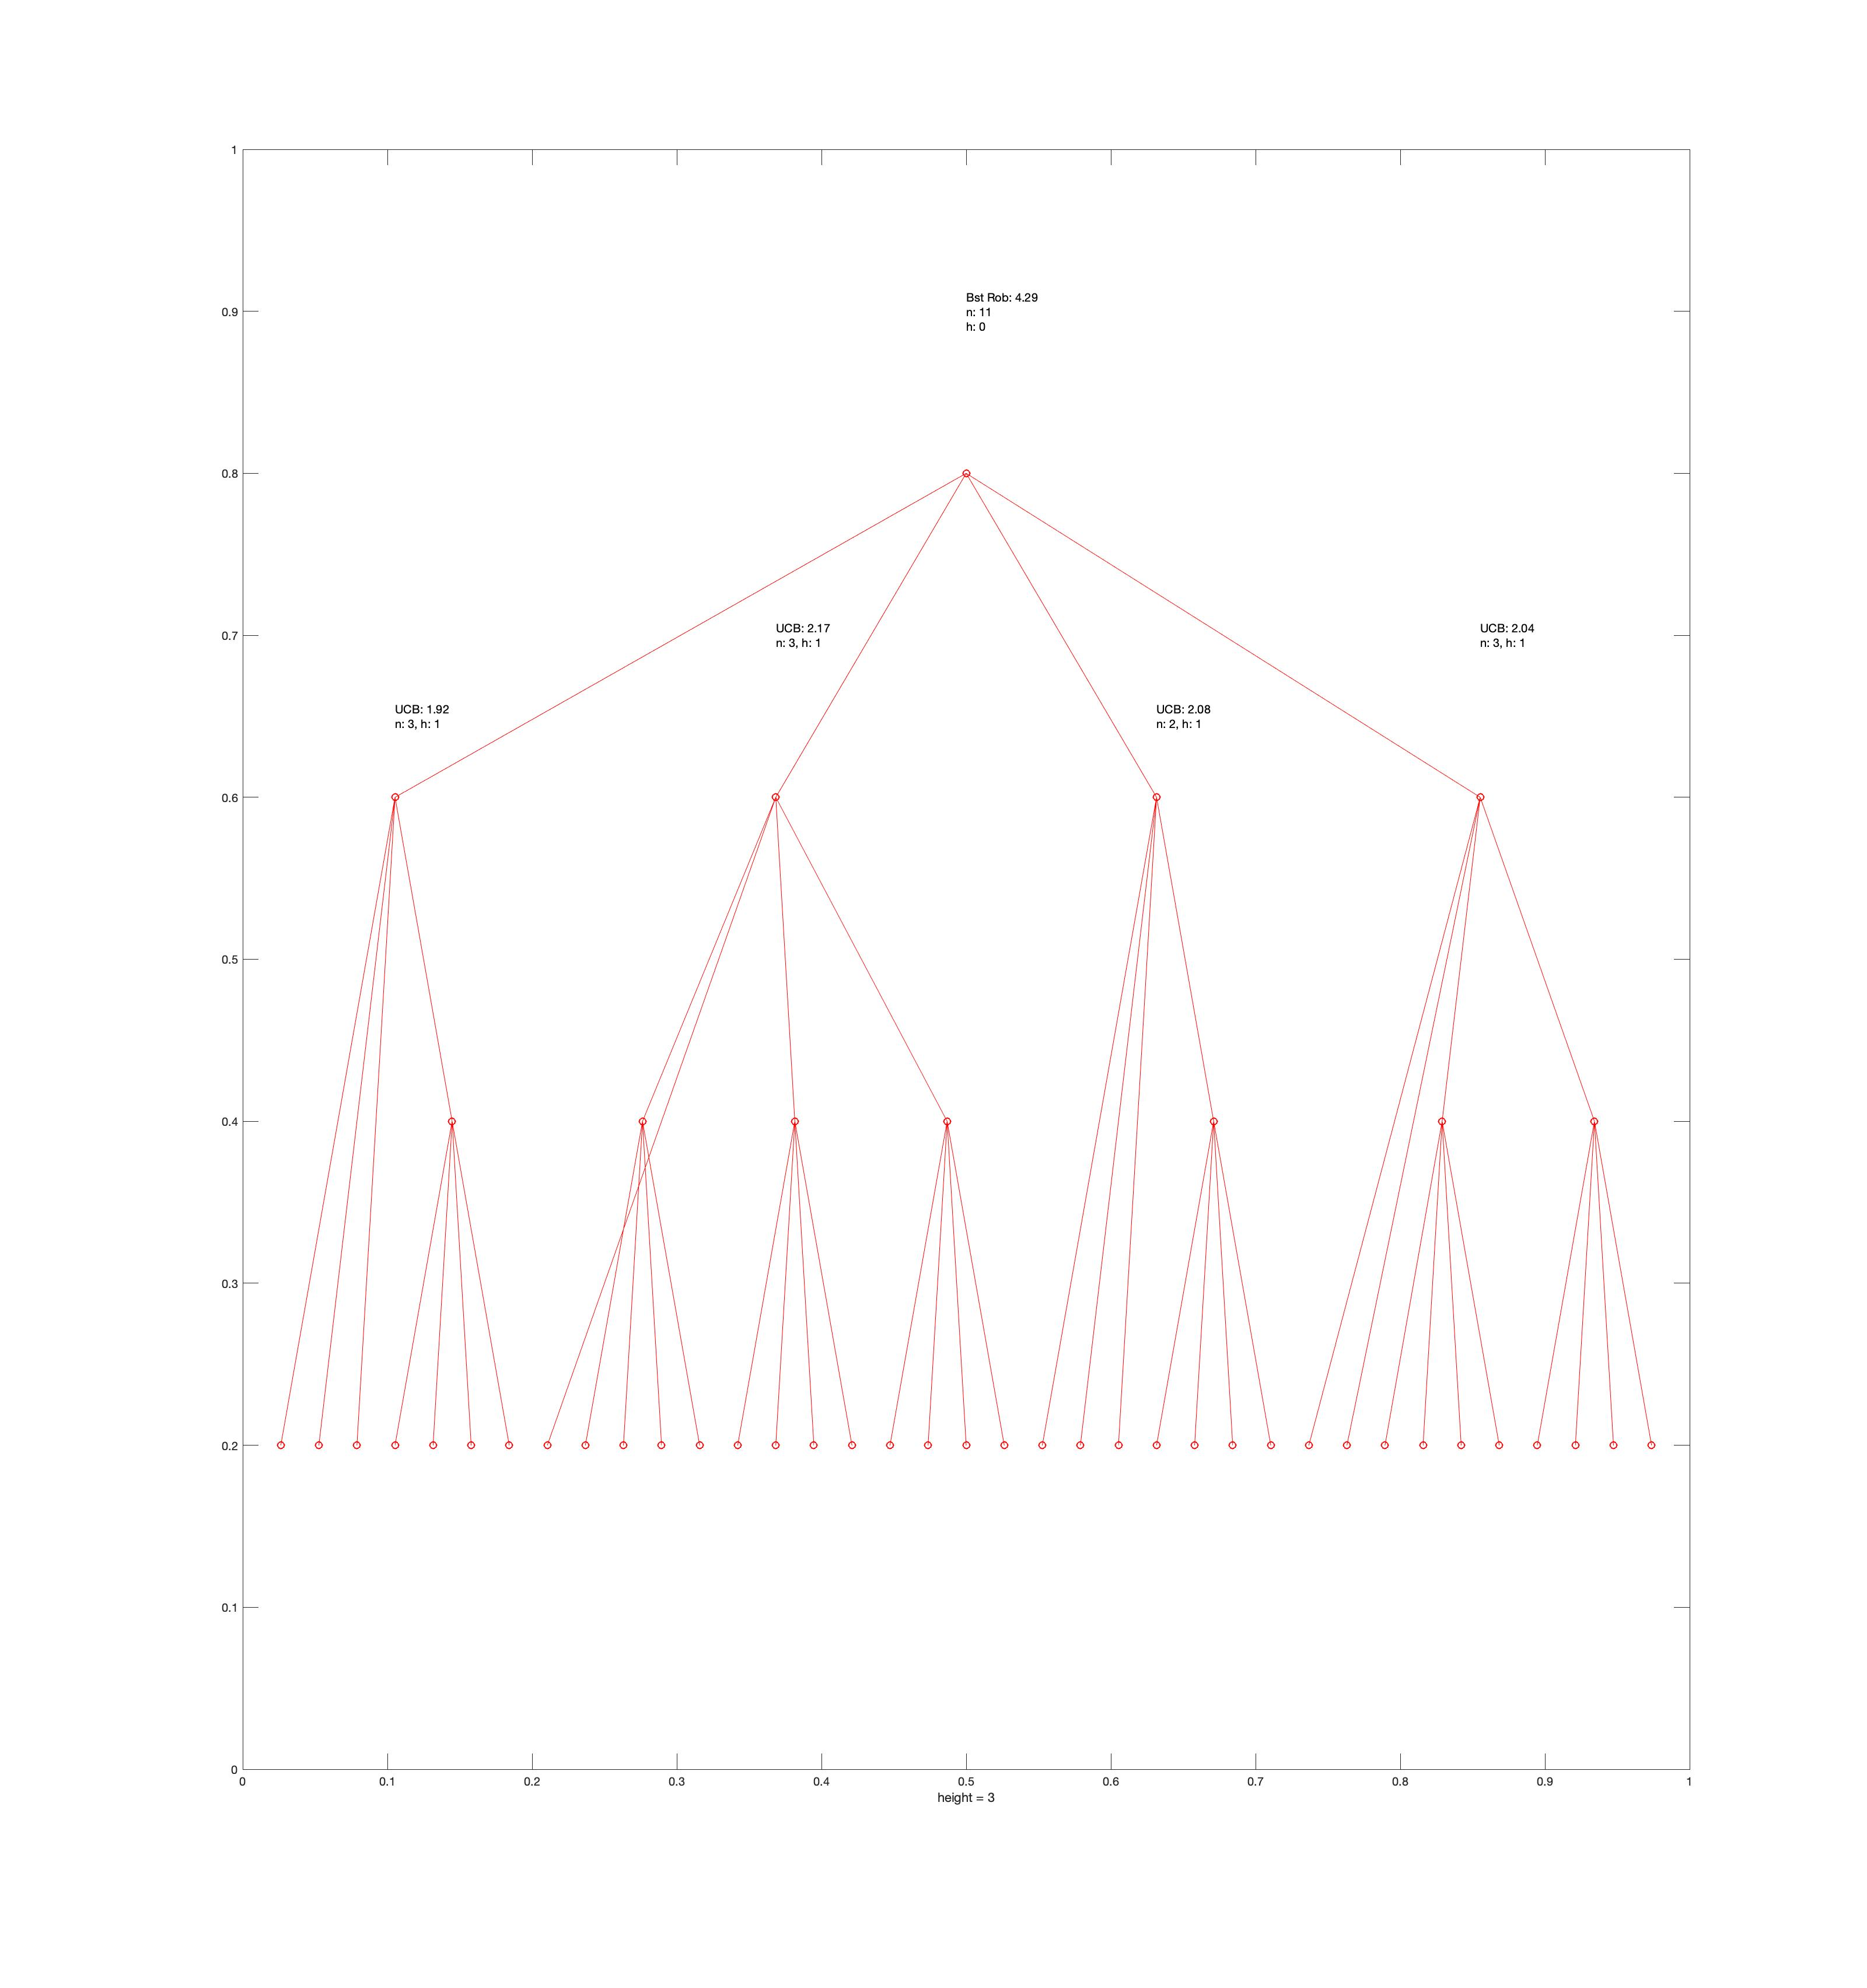
\includegraphics[width=\linewidth]{img/c1.jpg}
  \caption{MCTS: Favour exploration ($C=1$).}
  \label{fig:c1}
\end{figure}

\subsection{Lower-layer: Search Algorithms}~\label{sec:srcalg}
In the very end, the falsification task boils down to a search in the space of the states. 
We aim to find a falsifying trace of $k$ disturbances, where $k$ is the number of desired control points. 
To do so the MCTS (see Section~\ref{sec:MCTS}) when selects a node at depth $h$ to rollout from it, MCTS is basically defining a meta-trace $\hat{\delta}$. The first $h$ meta-disturb of $\hat{\delta}$ ($\hat{\delta}$ prefix) are regions of the input space in which to bound the search, and in the suffix the search is allowed in the whole input space. 

One of the following search algorithm is then used to produce a trace $\delta$ accordingly with the semantic of $\hat{\delta}$.

\subsubsection{Random Search: MCTS Left Alone}
To have a way to evaluate the contribution purely given by the MCTS layer, we decided to implement a fast yet dumb search strategy.
Given a meta-trace $\hat{\delta}$, for each control point $k$ in $\hat{\delta}$, RS basically samples u.a.r. a disturbance from the appropriate region for such control point.
This result in a very fast yet only exploring algorithm (see Section~\ref{sec:exp} for comparison). 

\subsubsection{Hill Climbing: the Greedy}
Here, the classical Hill Climbing implementation has been used. The only difference is that, since eventually we need a full trace (a trace having a disturbance for each control point), in the case a not worst neighbour isn't found at a given depth of the search, a random one is selected. 

Also, to have a stronger falsification power, at the cost of a longer simulation time restart has been implemented. 

On the other hand to speed up the simulation, at the cost of a weaker falsification power it is possible to bound the number of
neighbour tested by the algorithm at each step. 
Clearly this search strategy is way clever and effective than RS. Conversely, the simulation time needed to carry on the falsification process with a non trivial property to falsify is of another order of magnitude (see Section~\ref{sec:exp} for comparison).

\subsubsection{Simulated Annealing: the Impatient}
Again, classical search algorithm, basically an HC enriched with a notion of temperature or, as it is in this case, the MCTS budget (hence number of expanded nodes). The higher the temperature the hardest is to make a pejorative move. 
The goal here is to further balance exploration and exploitation and be, in terms of speed and performance in the middle of RS ans HC (see Section~\ref{sec:exp} for comparison).


\pagebreak

\section{Experimental phase}~\label{sec:exp}

\subsection{Model and Specifications}~\label{sec:exp:spec}
The benchmark adopted is the Automatic Transmission by MathWorks, provided in Simulink.
It models a vehicle equipped with a trasmission controller and allows the user to change two input signals:
the \textit{throttle} and the \textit{brake}.

There are several specifications defined on this model because it is a common benchmark in verification papers. Starting from the reference paper and \cite{bardh2014benchmarks}, we selected two           specification:

\begin{enumerate}
    \item The engine speed never reaches 120.
    \item If the vehicle gear is 3 then the speed is always greater than 20.
\end{enumerate}

We selected these two specifications because they are representative of different kind of search.
As explained in Section~\ref{sec:metic}, the first is easier to falsify as a greedy approach drives towards the decrease of robustness, the latter requires an higher exploration factor thus a more intelligent search.

\subsection{Implementation of Robustness Metric}~\label{sec:metic}
In order to undestand the difficulty of falsification of the second specification, we need to spend a few words on the computation of robustness metric used to drive the search.

According to the definition of Robustness given in\cite{fainekos2006robustness}, this metric gives us a measure of how the state of the model is far from the falsification. In the first specification,    the computation of Robustness is simply the difference between the reference speed and the current speed. Conversely, in the second specification the computation is more complex and can be summarized by  the following steps:

\begin{enumerate}
\item Since the second specification is an implication, we wrote it as an \texttt{OR}.
\item The Robustness of the \texttt{OR} operator is the max value of the Robustness computed in the two subformulas.
\item The first subformula is the absolute value of the difference between the current gear and the reference gear (3).
\item The second subformula is the difference between the current speed and the reference speed (20).
\end{enumerate}

Notice that the value of the second subformula is positive if the current speed is greater than 20, otherwise is negative. Conversely, the value of the first subformula is a small positive integer.

As a result, when the gear is different from the reference one (3) then the first subformula dominates the Robustness computation. When the gear is the third one, then the value could be dominated by     the second subformula only if it is greater than 20 and then positive. Then, the resulting metric space is characterized by long plateau when the current speed is far from 20 and local minima because of  the different unit of measurement for gear and speed.

\subsection{The proposed baseline: \texttt{URS}}
The two specifications above have been implemented in an external function in order to maintain a single model file. The Simulink model has been modified with two output blocks, respectively the \textit{speed} and the \textit{gear}. The external function computes the robustness according to the specification, described by a parameter in the configuration file.
\\ \\
The second specification S2 caused too long time to reach falsification and we decided to change its implementation in order to make it suitable to the time and resources that we can use. In particular, one of the main problem of S2 is the different units of measurment that lead to local minima. In fact, whilst speed is between 0 and 100, the gear is an integer value between 1 and 4.

In contrast with the original definition of the Robustness, we proposed to normalize the second subformula of S2 according to the unit scale. Since the speed goes from 0 to 100, we normalize the second subformula dividing by 100. In this way, the Robustness metric is still characterized by long plateau which make the search not trivial but we reduced the number of local minima.

\begin{figure}[h]
    \centering
    \textbf{Uniform Random Sampling - Robustness Distribution}\par
    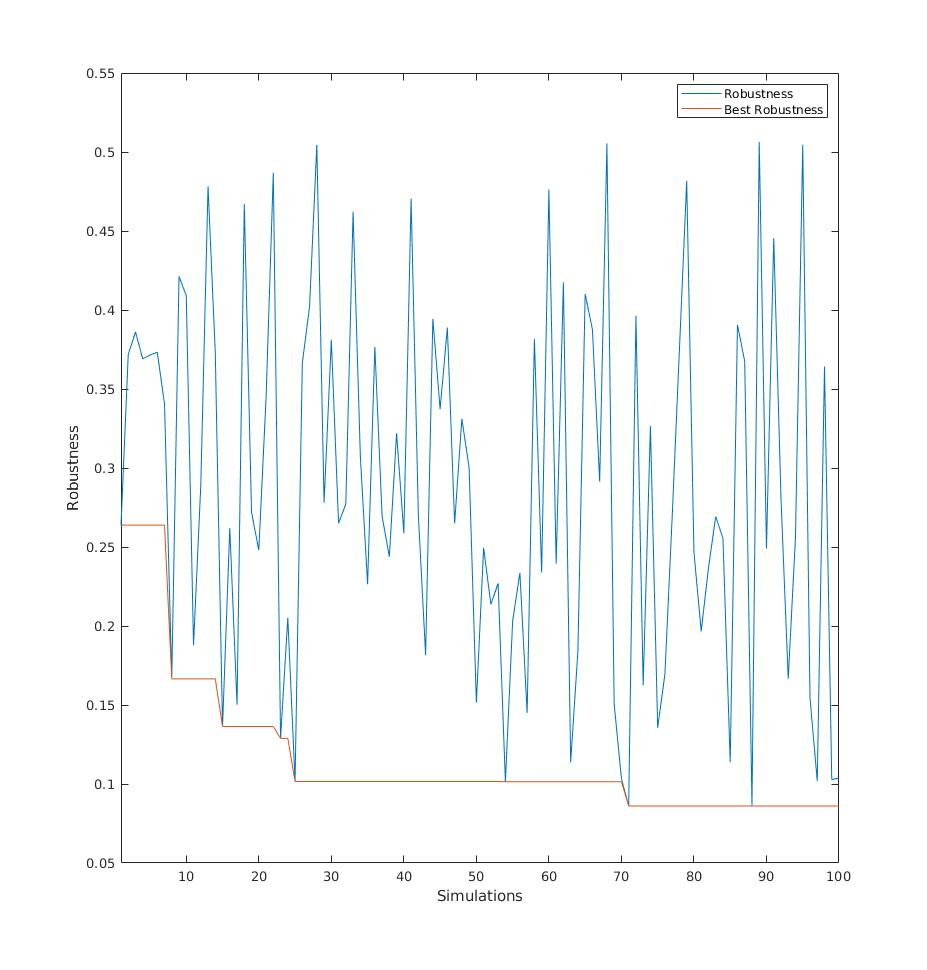
\includegraphics[width=0.5\linewidth]{img/urs_rob_distr.jpg}
    \caption{Robustness distribution over 100 simulation of URS search. This random distribution highlights that there is no learning in URS. Moreover, all the values are in [0,1] because we are using the normalized version of specific \texttt{S2} and is rather likely to reach the third gear at least once during the simulation with random values.}
\end{figure}

\pagebreak

\subsection{Experiments}~\label{sec:exp:exps}
In order to evaluate the effectiveness of the proposed falsification framework, we executed a bunch of experiments on the Automatic Transmission model considering several search algorithms: Uniform Random Sampling (URS), MCTS with Random Search (MCTS+RS), MCTS with Hill Climbing (MCTS+HC), MCTS with Simulated Annealing (MCTS+SA).

Since the execution of experiments is based on randomness, we repeated the same experiment 10 times to ensure more confident results.

First of all, we observed that the effectiveness of MCTS is based on its capacity to build the complete tree. In fact, the MCTS algorithm is characterized by a inherent phase of exploration which allows to have a general view of the space (tree width) and the time (tree height). Only when the tree is complete, the MCTS algorithm results effective and specializes the search.
As a consequence, if the branching factor of the nodes is too high, the number of simulation required to build the entire tree is huge and the MCTS doesn't result effective, compared with the URS. 

Thus, in order to exploit the power of MCTS, we tuned the split parameters for the input signals. The Speed signal has been split into 2 regions and the Brake signal has been split into 3 regions, then the branching factor of the tree is 6. In the original paper \cite{zhang2018two}, they
adopted a different tuning but we observed that such tuning is not effective compared with the URS algorithm. Moreover, for reason of time and resources, the experiments below have been configured with budget parameter equal to 100, it means that the maximum number of iterations of MCTS is 100 and then this is an upperbound in the number of simulations.

The tables below show the obtained results varying the parameter C which balance the value of exploration and exploitation in the UCB formula. The tables contain the following fields:
\begin{itemize}
    \item Algo: Search algorithm adopted.
    \item C: Value of parameter C.
    \item Avg Trace Falsification: Number of trace before falsification, considering only the tests which falsify the specification.
    \item Success Rate: Number of tests which falsify the specification.
    \item Robustness: statistics on robustness value.
    \item Time: statistics on elapsed time, both time are considered as average of the all number of experiments.
\end{itemize}

Furthermore, the results varying the input space partitioning are reported in the Table~\ref{table:patitioning} in order to emphasize the influence of hyperparameter tuning.

In order to highlights the different approach of search algorithms adopted, the Figure~\ref{img:rob_monitoring} shows the Robustness over the experiments of a sample of 5 experiments. For each search algorithm MCTS+RS, MCTS+HC, MCTS+SA, the Figure represent what has been the Robustness obtained and the current best Robustness. Moreover, the Figure shows in the first half the experiments with $C=0.0$ and in the second half the experiments with $C=0.125$. In this way, it also highlights the impact of MCTS exploration/exploitation factor on the search algorithm underlying.

% TEST ON SPEC 1
\begin{table}[ht]
\centering
\title{Experiments on specification \texttt{S1}}
\begin{tabular}{|l|l|c|c|c|c|c|c|c|}
\hline
\multicolumn{1}{|c|}{\multirow{2}{*}{Algo}} & \multirow{2}{*}{C} & Avg Trace               & \multirow{2}{*}{Success Rate} & \multicolumn{3}{c|}{Robustness} & \multicolumn{2}{c|}{Time (sec)} \\ \cline{5-9} 
\multicolumn{1}{|c|}{}                      &                    & Falsification           &                               & min       & avg      & std dev  & tot        & trace        \\ \hline
URS                                         & - - -              &  40.0                   & 2/10                          & -4.07960  & 4.91882  & 5.514537 &  178.014 &  2.010    \\ \hline
MCTS+RS                                     & 0.500              & - - -                   & 0/10                          &  5.30248  & 8.34921  & 2.400517 &  559.916 &  5.599    \\
MCTS+HC                                     & 0.500              &  94.0                   & 1/10                          & -1.93401  & 5.07959  & 4.386757 & 1034.225 & 10.405    \\
\textbf{MCTS+SA}                                     & \textbf{0.500}              &  \textbf{24.0}                   & \textbf{1/10}                          & \textbf{-0.68394}  & \textbf{7.71311}  & \textbf{4.152730} &  \textbf{891.788} &  \textbf{9.781}    \\ \hline

MCTS+RS                                     & 0.250              &  62.0                   & 4/10                          & -4.52952  &  2.80386 & 4.995340 &  355.163 &  4.198    \\
MCTS+HC                                     & 0.250              &  74.4                   & 5/10                          & -3.63763  &  2.02058 & 4.289398 &  676.262 &  7.774    \\
\textbf{MCTS+SA}                                     & \textbf{0.250}              &  \textbf{74.6}                   & \textbf{7/10}                          & \textbf{-10.29078} & \textbf{-2.38069} & \textbf{3.744391} &  \textbf{597.866} &  \textbf{7.297}    \\ \hline

\textbf{MCTS+RS}                                     & \textbf{0.125}              &  \textbf{46.5}                   & \textbf{8/10}                          & \textbf{-6.27352}  & \textbf{-1.28520} & \textbf{3.320830} &  \textbf{170.078} &  \textbf{2.996}    \\
MCTS+HC                                     & 0.125              &  68.1                   & 8/10                          & -4.61933  & -0.07330 & 4.719893 &  380.664 &  5.127    \\
MCTS+SA                                     & 0.125              &  48.5                   & 8/10                          & -6.43350  & -0.69363 & 5.875865 &  304.758 &  5.225    \\ \hline

MCTS+RS                                     & 0.000              &  65.5                   & 2/10                          & -4.20689  & 6.83323  & 7.070816 &  325.054 &  3.510    \\
\textbf{MCTS+HC}                                     & \textbf{0.000}              &  \textbf{41.0}                   & \textbf{4/10}                          & \textbf{-2.64884}  & \textbf{1.95654}  & \textbf{3.712926} &  \textbf{430.037} &  \textbf{5.589}    \\
MCTS+SA                                     & 0.000              &  78.0                   & 2/10                          & -1.51834  & 4.81908  & 6.613282 &  558.383 &  5.834    \\ \hline
\end{tabular}
\caption{Comparison between MCTS and URS, given a budget of 100 simulations and varying the parameter C in order to balance exploration and exploitation in the search. The input signals have been split into 2 and 3 region.}~\label{table:res:s1}
\end{table}

% TEST ON SPEC 2
\begin{table}[ht]
\centering
\title{Experiments on specification \texttt{S2}}
\begin{tabular}{|l|l|c|c|c|c|c|c|c|}
\hline
\multicolumn{1}{|c|}{\multirow{2}{*}{Algo}} & \multirow{2}{*}{C} & Avg Trace               & \multirow{2}{*}{Success Rate} & \multicolumn{3}{c|}{Robustness} & \multicolumn{2}{c|}{Time (sec)} \\ \cline{5-9} 
\multicolumn{1}{|c|}{}                      &                    & Falsification           &                               & min      & avg      & std dev  & tot        & trace        \\ \hline
URS                                         & - - -              & - - -                   & 0/10                          & 0.02080  & 0.06130  & 0.03130  &  408.585   &  4.086       \\ \hline
MCTS+RS                                     & 0.500              &  90.0                   & 2/10                          & 0.00000  & 0.05430  & 0.04420  &  397.635   &  4.056       \\
\textbf{MCTS+HC}                                     & \textbf{0.500}              &  \textbf{53.0}                   & \textbf{7/10}                          & \textbf{0.00000}  & \textbf{0.00490}  & \textbf{0.00840}  & \textbf{1039.426}   & \textbf{15.517}       \\
MCTS+SA                                     & 0.500              & - - -                   & 0/10                          & 0.00071  & 0.04930  & 0.04330  &  681.465   &  6.815       \\ \hline

MCTS+RS                                     & 0.250              & - - -                   & 0/10                          & 0.00661  & 0.03571  & 0.02372  &  572.351   &  5.723       \\
\textbf{MCTS+HC}                                     & \textbf{0.250}              &  \textbf{29.1}                   & \textbf{9/10}                          & \textbf{0.00000}  & \textbf{0.00023}  & \textbf{0.00073}  &  \textbf{914.175}   & \textbf{26.076}       \\
MCTS+SA                                     & 0.250              &  46.0                   & 1/10                          & 0.00000  & 0.06933  & 0.09205  &  941.542   &  9.977       \\ \hline

MCTS+RS                                     & 0.125              &  42.7                   & 3/10                          & 0.00000  & 0.04101  & 0.03548  &  275.017   &  3.325       \\
\textbf{MCTS+HC}                                     & \textbf{0.125}              &  \textbf{31.6}                   & \textbf{8/10}                          & \textbf{0.00000}  & \textbf{0.00388}  & \textbf{0.00843}  &  \textbf{497.749}   & \textbf{11.466}       \\
MCTS+SA                                     & 0.125              &  76.3                   & 4/10                          & 0.00000  & 0.05349  & 0.11098  &  506.049   &  5.577       \\ \hline

MCTS+RS                                     & 0.000              &  32.0                   & 1/10                          & 0.00000  & 0.14757  & 0.16817  &  473.518   &  5.113       \\
\textbf{MCTS+HC}                                     & \textbf{0.000}              &  \textbf{36.6}                   & \textbf{5/10}                          & \textbf{0.00000}  & \textbf{0.01148}  & \textbf{0.01682}  & \textbf{1322.240}   & \textbf{19.317}       \\
MCTS+SA                                     & 0.000              & - - -                   & 0/10                          & 0.00834  & 0.16304  & 0.14714  &  873.488   &  8.734       \\ \hline
\end{tabular}
\caption{Comparison between MCTS and URS, given a budget of 100 simulations and varying the parameter C in order to balance exploration and exploitation in the search. The input signals have been split into 2 and 3 region.}~\label{table:res:s2}
\end{table}

% TEST ON SPEC 2 comparing partitioning
\begin{table}[ht]
\centering
\title{Experiments on different partitioning}
\begin{tabular}{|l|l|c|c|c|c|c|c|c|}
\hline
\multicolumn{1}{|c|}{\multirow{2}{*}{Algo}} & \multirow{2}{*}{Part} & Avg Trace               & \multirow{2}{*}{Success Rate} & \multicolumn{3}{c|}{Robustness} & \multicolumn{2}{c|}{Time (sec)} \\ \cline{5-9} 
\multicolumn{1}{|c|}{}                      &                    & Falsification           &                               & min      & avg      & std dev  & tot        & trace        \\ \hline
URS                                         & - - -              & - - -                   & 0/10                          & 0.02080  & 0.06130  & 0.03130  &  408.585   &  4.086       \\ \hline
MCTS+RS                                     & 2x3                &  90.0                   & 2/10                          & 0.00000  & 0.05430  & 0.04420  &  397.635   &  4.056       \\
\textbf{MCTS+HC}                                     & \textbf{2x3}                &  \textbf{53.0}                   & \textbf{7/10}                          & \textbf{0.00000}  & \textbf{0.00490}  & \textbf{0.00840}  & \textbf{1039.426}   & \textbf{15.517}       \\
MCTS+SA                                     & 2x3                & - - -                   & 0/10                          & 0.00071  & 0.04930  & 0.04330  &  681.465   &  6.815       \\ \hline

MCTS+RS                                     & 2x2                &  70.0                   & 3/10                          & 0.00000  & 0.06517  & 0.06197  &  631.963   &  6.804       \\
\textbf{MCTS+HC}                                     & \textbf{2x2}                &  \textbf{48.7}                   & \textbf{7/10}                          & \textbf{0.00000}  & \textbf{0.00099}  & \textbf{0.00163}  & \textbf{1479.660}   & \textbf{22.530}       \\
MCTS+SA                                     & 2x2                & - - -                   & 0/10                          & 0.00561  & 0.05776  & 0.02567  & 1393.552   & 13.936       \\ \hline
\end{tabular}
\caption{Comparison of search algo with fixed C=0.5 and varying the input space partitioning. Test on spec \texttt{S2}.}~\label{table:patitioning}
\end{table}

\pagebreak

\section{Analysis of the results}~\label{sec:resan}
In this section, a contextual analysis of the experimental results and of what are the factors which influenced such results.
Before analysing the results, we enforce that many problems have been overcome in order to obtain and evaluate the proposed approach. 

For example, randomness in Matlab is not always random as one would expect. In fact, at every startup the seed which generate the random sequence is the same, thus we had to further tweak the environment in order to avoid the risk to select a favorable configuration. Moreover, the object orientation in poorly handled in Matlab, especially when you decide to use a Simulink model. In fact, we faced with problems and poor performances caused by scope overloading. To solve these
problems, we had to rewrite the all code avoiding object-orientation and only using scripts and global scopes. We did all our best to give structure and cleanless to the code using packages and structs. 
% In order to evauate the system proposed different test has been deviced and executed.

\subsection{Comments}
The first experiments presented consider a fixed input space partitioning (2x3) and have been tested on both specifications \texttt{S1} and \texttt{S2}, varying the parameter $C$.

% \subsubsection{S1}
\paragraph{S1} \textit{The engine speed never reaches 120}. Clearly the robustness function resulting by \texttt{S1} is proportional to the break signal and inversely proportional to throttle, \textit{i.e.} high value of throttle and low value of brake lead to low robustness.
As a consequence, minimizing the robustness should be quite straightforward, even using a greedy search, such as Hill Climbing.

According to this intuition, the best performing experiments are those with a reasonably small value for $C=0.125$, as you ca see in Table~\ref{table:res:s1}.
Recall that a small $C$ means give a bias towards exploitation rather than exploration. Thus, encouraging the exploitation reflects the monotonic nature of the robustness of \texttt{S1} and then exploiting promising regions gives back promising results.

The results obtained by MCTS and Hill Climbing (MCTS+HC) represent another evidence of this intuition. Furthermore, the computational overhead due to the Hill Climbing search is almost negligible. The reason is that the search proceeds almost straight, following the steepest hill of the robustness curve and then Hill Climbing easily finds not pejorative neighbour. 

Conversely, favouring exploration (\textit{e.g.} $C=0.5$) results in extremely poor results. In fact, the falsification rate is even worst than \texttt{URS} and the reason is that most of the budget is wasted in the exploration of the huge state space. Moreover, the overhead of Hill Climbing (MCTS+HC) and Simulated Annealing (MCTS+SA) is quite relevant because exploration of less promising regions leads to difficulties in finding not pejorative neighbours (MCTS+HC presents a net 2x overhead).

\paragraph{S2} \textit{If the vehicle gear is 3 then the speed is always greater than 20}.
As already said in the Section~\ref{sec:exp:spec}, this specification is not trivial at all and a clever strategy is needed in order to do any falsification.
Evidence of this is the fact that Uniform Random Sampling (URS) is never able to falsify such requirement, as can be observed from Table~\ref{table:res:s2}.

The best performing strategy here is again MCTS and Hill Climbing (MCTS+HC), which is able to falsify \texttt{S2} specification $9$ times out of $10$ with $C=0.25$.

Note that:
\begin{itemize}
    \item The $C$ hyper-parameter balances two factors, exploitation and exploitation.
    \item The exploration factor is not normalized, typically is $\in [0,2.5]$.
    \item The exploitation is normalized $\in [0,1]$.
\end{itemize}
The ratio among the two factors is in the order of $2.5$. Then, using $C=0.25$, this ratio is mapped into a more reasonable and performing $0.6$ factor which favours exploitation and maintains exploration.

Finally, in the experiments which falsify the specification, the number of simulated trace is surprisingly small, as reported by the column \textit{Avg Trace Falsification}. This is due the effectiveness of the search algorithm and highlights their performance.

\paragraph{Impact of search algorithms.}
The previous comments consider the obtained result in a monolithic way, without any consideration of the two-layers search. Considering the details about the Robustness distribution varying the search algorithm allows to understand what is the impact of each search algorithm in the lower level. For this reason, we reported a sample of 5 tests in the Figure~\ref{img:rob_monitoring} varying the search algorithm and presenting the result with $C=0.0$ (worst performance) and $C=0.125$ (best performance).

First of all, in both the experiments, we can observe a different behaviour between MCTS+HC and MCTS+RS, MCTS+SA. Whilst MCTS+HC remains bounded locally with respect to the Robustness value, the other search algorithms present high peaks. These wide oscillations correspond with a less effective search that has been confirmed by the results.

Considering the experiments with $C=0.0$, all the algorithms seem to explore their best regions without any exploration and for this reason, they rarely reach the falsification. Even the MCTS+HC continue to search locally without success (3 times over 5). However, when MCTS+HC luckily choose the right down-hill, it go straight and reach falsification (2 times over 5).

Conversely, considering the best tuning with $C=0.125$, all the algorithms perform better than the previous experiments. The peculiar behaviour of each algorithm is confirmed. In fact, we can easily recognize the shape of the MCTS+HC compared with the others.

\begin{figure}[H]~\label{img:rob_monitoring}
    \centering
    \textbf{Robustness Monitoring - Test with C=0.0}\par
    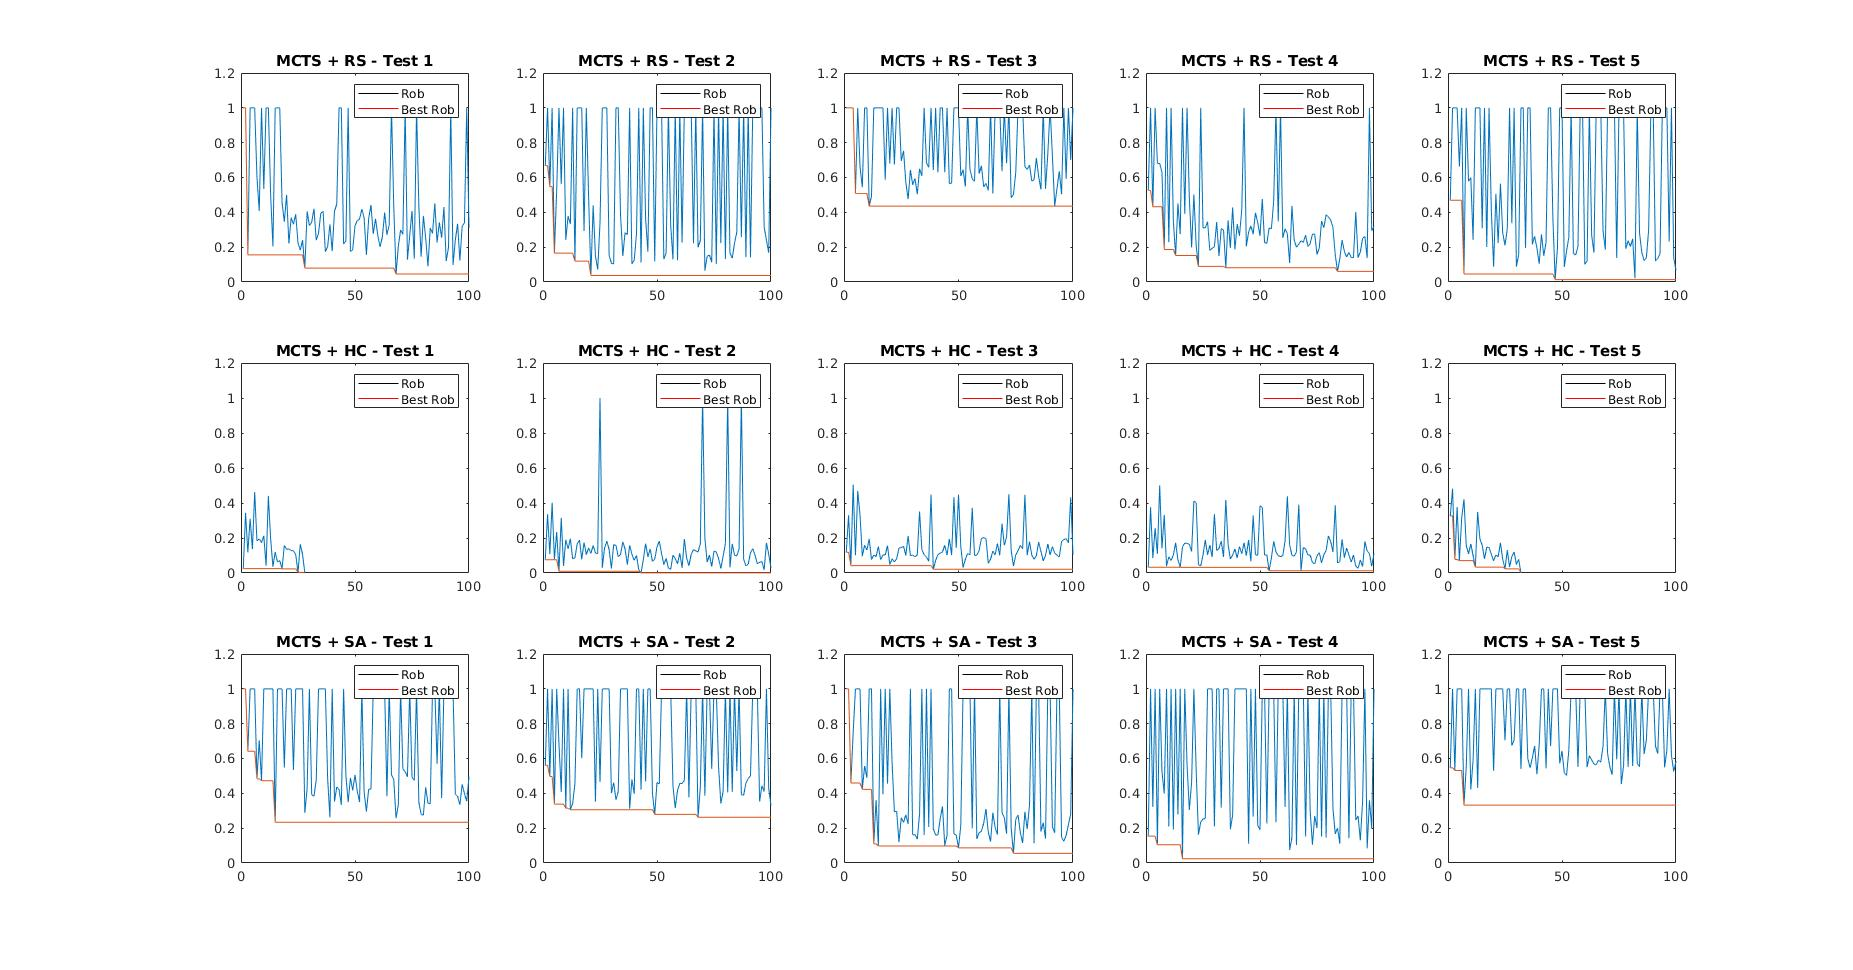
\includegraphics[width=\linewidth]{img/0_000/compare_search_rob_blue.jpg}

    \textbf{Robustness Monitoring - Test with C=0.125}\par
    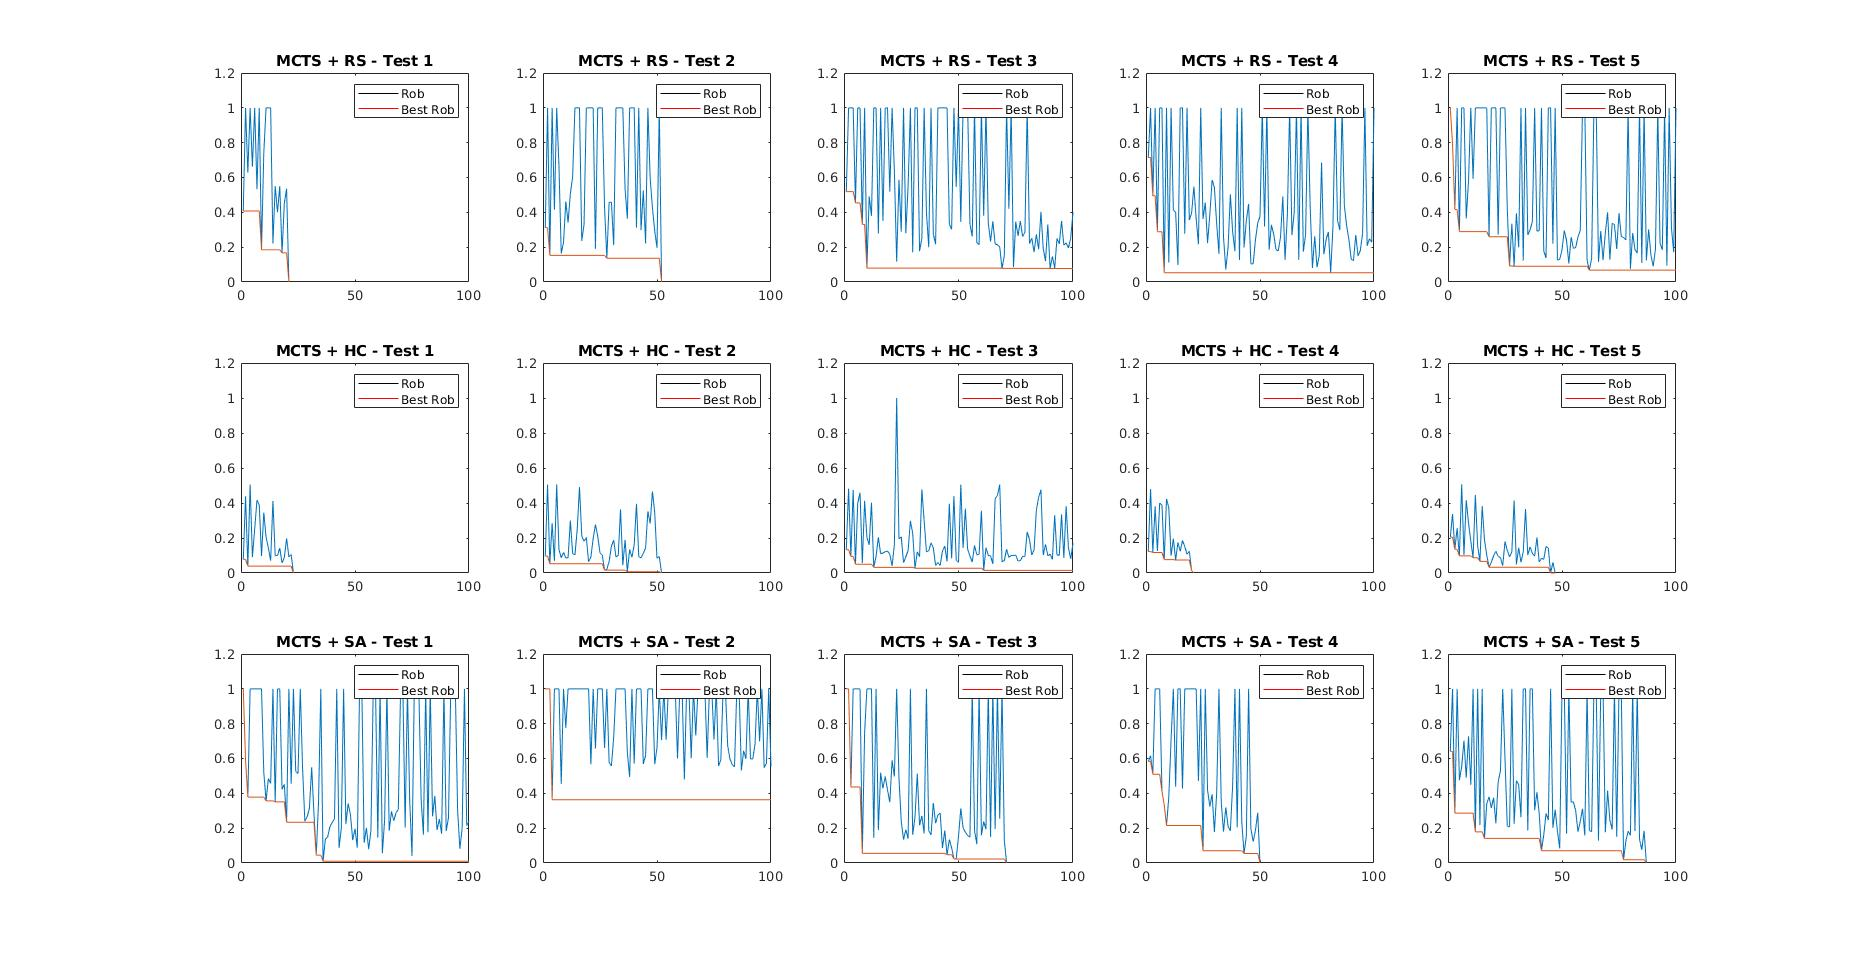
\includegraphics[width=\linewidth]{img/0_125/compare_search_rob_blue_orange.jpg}
    \caption{Comparison of robustness monitoring using different search algorithm: MCTS+RS (first line), MCTS+HC (second line), MCTS+SA (third line). Robustness distribution over 100 simulation, picking 5 sample test of falsification on specification \texttt{S2}.}
\end{figure}

\paragraph{Execution Times}
In conclusion, a brief consideration of the execution time is worth to be made.
However, even if the performances for Hill Climbing are quite good even for this non-trivial specification, they come with a higher cost. The \textit{Time} column of Table~\ref{table:res:s2} highlights that the time needed to simulated a single trace with MCTS+HC is $26.076$ seconds, compared with $5.723$ seconds needed for MCTS+RS and $9.977$ seconds for MCTS+SA.
Having a cluster of multiple machines would allow to test multiple configuration of the same experiment and exploit \textit{a posteriori} those configurations which expand the tree, pruning those configurations which waste time on not relevant regions. 

Comparing the times of the several MCTS implementations with the Uniform Random Sampling (\texttt{URS}), one can notice that the overhead of MCTS layer is minimal. In fact, the difference between the overall times for URS and MCTS+RS is not relevant and then, we can conclude that the upper layer is performed with a little overhead. 
Unfortunately, this is only true when using Random Sampling as search algorithm. Any other search algorithm ends up in a more consistent overhead, after all \textit{there is no free lunch}. 

\paragraph{State Space Partitioning}
Table~\ref{table:patitioning} show another direction of tests we investigated on. In such experiment, the state space is partitioned in a different way: the throttle and the brake has been divided into two regions (2x2) or in two and three regions respectively (2x3), as in the previous experiments.
This may sound as a pointless modification but it opens up the scenario described till now to a new perspective.
This new partitioning induces a MCTS tree with a smaller branching factor ($4$ vs $6$). Direct consequences are the following:
\begin{enumerate}
    \item The space partitioning is coarse grained.
    \item MCTS has an higher view of the search space.
    \item Lower branching factor allow the MCTS to finish earlier the tree building.
    \item The effort is moved to the search algorithm in the rollout phase.
\end{enumerate}

The experiments done are only a few and still far to a conclusion. However, they produce a slight improvement in Falsification Rate as well as Avg Trace Falsification. This fact sheds the light on the importance of hyper-parameter tuning because it could lead to a relevant boost in performances (see Section~\ref{sec:hp}).

%TODO: add plot of robustness function vs trace found (quello che abbiamo mostrato al proff)
%TODO: table with results and plot for robustnes and graph

\subsection{Hyperparameters}~\label{sec:hp}
As already remarked, the role of hyper-parameters and the importance of a proper tuning of those is crucial for effectiveness of search algorithm.
Having the computational power to do so, a proper grid search in the space of hyper-parameter should be performed to fine-tune the system and fully exploit its potentiality.
The hyper-parameters that should be investigated are the following:
\begin{enumerate}
    \item C: in order to balance exploration and exploitation and to better combine MCTS with a given search strategy.
    \item Space partitioning: in order to control MCTS branching factor.
    \item Disturbance quantization: in order to control the search space and to avoid its explosion.
    \item Control Points: in order to define the degree of freedom of the simulation itself.
\end{enumerate}
Clearly a full search is prohibitive thus a clever approach should be devised in order to performs hyper-parameters optimization.

\section{Conclusion}
In this project, we had the chance to explore a new trend in falsification which consists of the application of a sophisticated combination of search algorithms in falsification of Temporal Logic specifications. The proposed MCTS algorithm performs well, even in more challenging scenario as the Specification \texttt{S2}, but it shown that it requires a high number of simulation to compute the search tree because the building is based on exploration of each branch. As a consequence, the application of MCTS on simple specifications (\textit{i.e. easy to find an event trace which falsify the specification}) doesn't result effective.

In conclusion, we would like to propose a few developments of the presented work:
\begin{enumerate}
    \item Since the tuning of parameter $C$ seems to be determinant, an extension of the algorithm could be its adaptive version which change the value of $C$ according to the obtained results. The design of a learning model could be explored with a reinforcement learning approach. 
    \item The proposed approach doesn't take into account any domain knowledge that could be exploited on a specific model. In fact, we could customize:
        \begin{enumerate}
            \item the ordering of node explored in the Expansion phase. We could infer an ordering to bias toward know-to-be-good regions.
            \item the branching factor at different levels of tree because the height of the tree corresponds to the time advancement. We could adopt a low branching factor in less significant period of time and a wide branching factor on more interesting time periods.
        \end{enumerate}
    \item The adopted UCB formula seems to be a bias towards exploration because the two terms are not normalized properly. In fact, the first term is normalized in [0,1] whilst the second term is not and change in [0,3]. We could rafine this formula normalizing the second term with respect to the max value, improving the performance.
    \item The tree structure of MCTS seems to be adapt to a parallel execution. In particular, the expansion phase at a given layer will expand all node with a 0 score and up till exist a 0 score node a node with such score is selected, it is possible to exploit embarrassing parallelism with a master-slave architecture to speed up the expansion phase which is the bottle neck of MCTS. That way, one layer can be attacked at once to reduce the exploration cost and invest in exploration. 
\end{enumerate}

The system presented, which eventually obtains good performances, could largely benefits from all these new directions.


\bibliographystyle{plain}
\bibliography{biblio}

\end{document}
